%----------------------------------------------------------------------------------------
%	PACKAGES AND THEMES
%----------------------------------------------------------------------------------------
\documentclass{beamer}
\usepackage[utf8]{inputenc}

\usetheme{Boadilla}
\usecolortheme{default}
\setbeamertemplate{navigation symbols}{}%remove navigation symbols

\usepackage{amsmath}
\usepackage{amssymb}
\usepackage{amsthm}
\usepackage{hyperref}
\usepackage{graphicx} % Allows including images
\usepackage{booktabs} % Allows the use of \toprule, \midrule and \bottomrule in tables

%----------------------------------------------------------------------------------------
%	TITLE PAGE
%----------------------------------------------------------------------------------------

% The title
\title{Origami konstrukcije in reševanje problemov s prepogibanjem papirja}

\author{Terezija Krečič}
\institute[FMF] % Your institution may be shorthand to save space
{
    % Your institution for the title page
    Mentor: prof.~dr.~Aleš Vavpetič
    \vskip 3pt
    Fakulteta za matematiko in fiziko \\
    Pedagoška matematika
    \vskip 3pt
}
\date{{22.\ maj 2025}} % Date, can be changed to a custom date



% ROČNO nastavljeni footerji (avtor + podnaslovi)
\setbeamertemplate{footline}
{%
  \leavevmode%
  \hbox{%
  \begin{beamercolorbox}[wd=.25\paperwidth,ht=2.25ex,dp=1ex,center]{author in head/foot}%
    \usebeamerfont{title in head/foot}\insertauthor
  \end{beamercolorbox}%
  \begin{beamercolorbox}[wd=.75\paperwidth,ht=2.25ex,dp=1ex,leftskip=2ex,rightskip=2ex,sep=0pt]{date in head/foot}%
    \insertsectionhead%
    \hfill%
    \usebeamercolor[fg]{page number in head/foot}%
    \usebeamerfont{page number in head/foot}%
    \usebeamertemplate{page number in head/foot}%
  \end{beamercolorbox}}%
  \vskip0pt%
}
%----------------------------------------------------------------------------------------
%	PRESENTATION SLIDES
%----------------------------------------------------------------------------------------

\begin{document}

\begin{frame}
    % Print the title page as the first slide
    \titlepage
\end{frame}

\begin{frame}{Pregled}
    % Throughout your presentation, if you choose to use \section{} and \subsection{} commands, these will automatically be printed on this slide as an overview of your presentation
    \tableofcontents
\end{frame}

%------------------------------------------------
\section{Osnovna literatura}
%------------------------------------------------

\begin{frame}{Osnovna literatura}
    \begin{figure}[h]
        \centering
        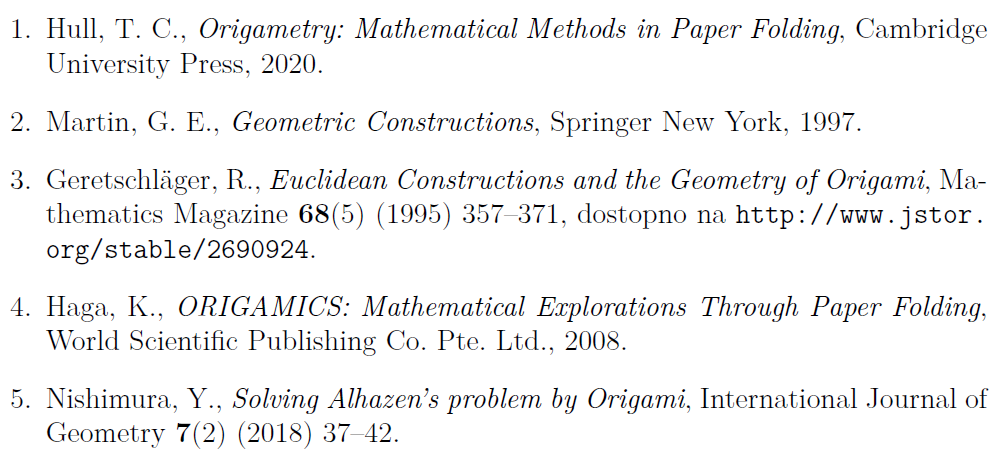
\includegraphics[width=\textwidth]{images/osnovna_literatura.png}
    \end{figure}
\end{frame}

%------------------------------------------------


%------------------------------------------------
\section{Origami konstrukcije}
%------------------------------------------------

\begin{frame}{Origami operacije}
    Pravila prepogibanja:
    \begin{itemize}
        \item enkratni in ravni pregibi
        \item dodatna orodja
    \end{itemize}
    Vsi možni pregibi:
    \begin{figure}[h]
        \centering
        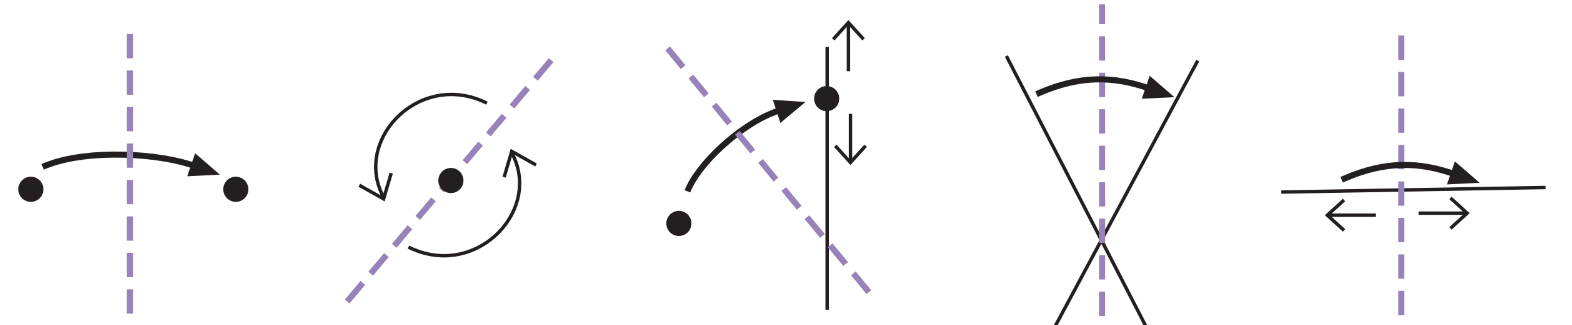
\includegraphics[width=0.9\textwidth]{images/hull_vsi pregibi.png}
    \end{figure}
    Origami operacije O1--O8.
\end{frame}

%------------------------------------------------

\begin{frame}{}
    \begin{alertblock}{Izrek $2.7$}
        Če dovolimo le enkratne in ravne pregibe, so edine možne operacije prepogibanja operacije O1--O8.
    \end{alertblock}
    \begin{alertblock}{Trditvi $2.10$ in $2.11$}
        Z ravnimi in enkratnimi prepogibi ter upoštevanjem origami operacij lahko s prepogibanjem papirja zrcalimo točke in prenašamo razdalje.
    \end{alertblock}
    \begin{figure}[h]
        \centering
        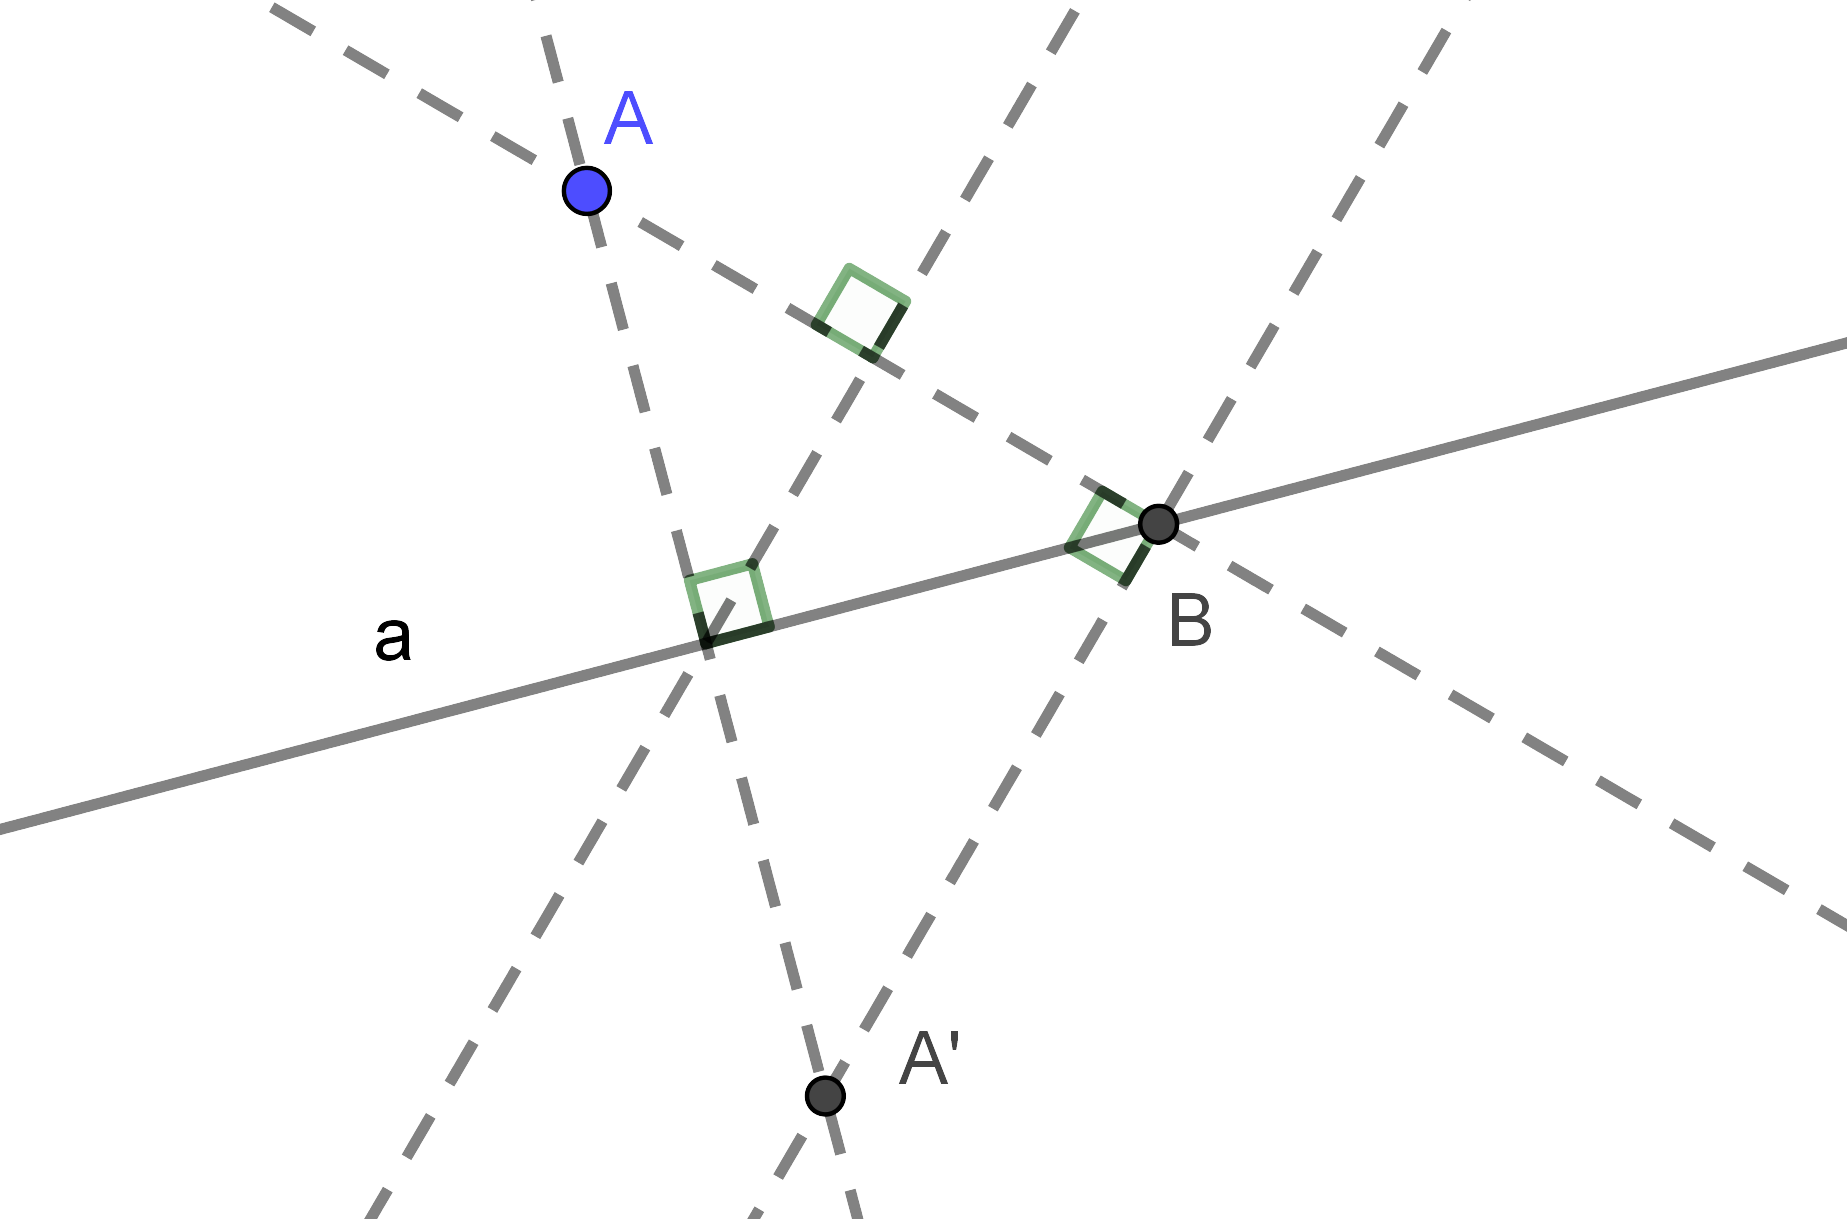
\includegraphics[width=0.4\textwidth]{images/zrcaljenje_tocke_cez_premico.png}
        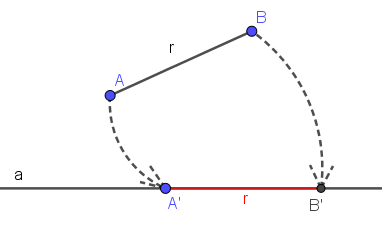
\includegraphics[width=0.4\textwidth]{images/zrcaljenje_konec.png}
    \end{figure}
\end{frame}

%------------------------------------------------

\begin{frame}{$\mathbb{O}$: množica origami števil}
    \begin{alertblock}{Izrek $2.29$ in trditev $2.30$}
        Množica $\mathbb{O}$ je podpolje polja $\mathbb{C}$. Za $\alpha \in \mathbb{O}$ velja $\sqrt{\alpha}, \sqrt[3]{\alpha} \in \mathbb{O}$.
    \end{alertblock}
    \begin{figure}[h]
        \centering
        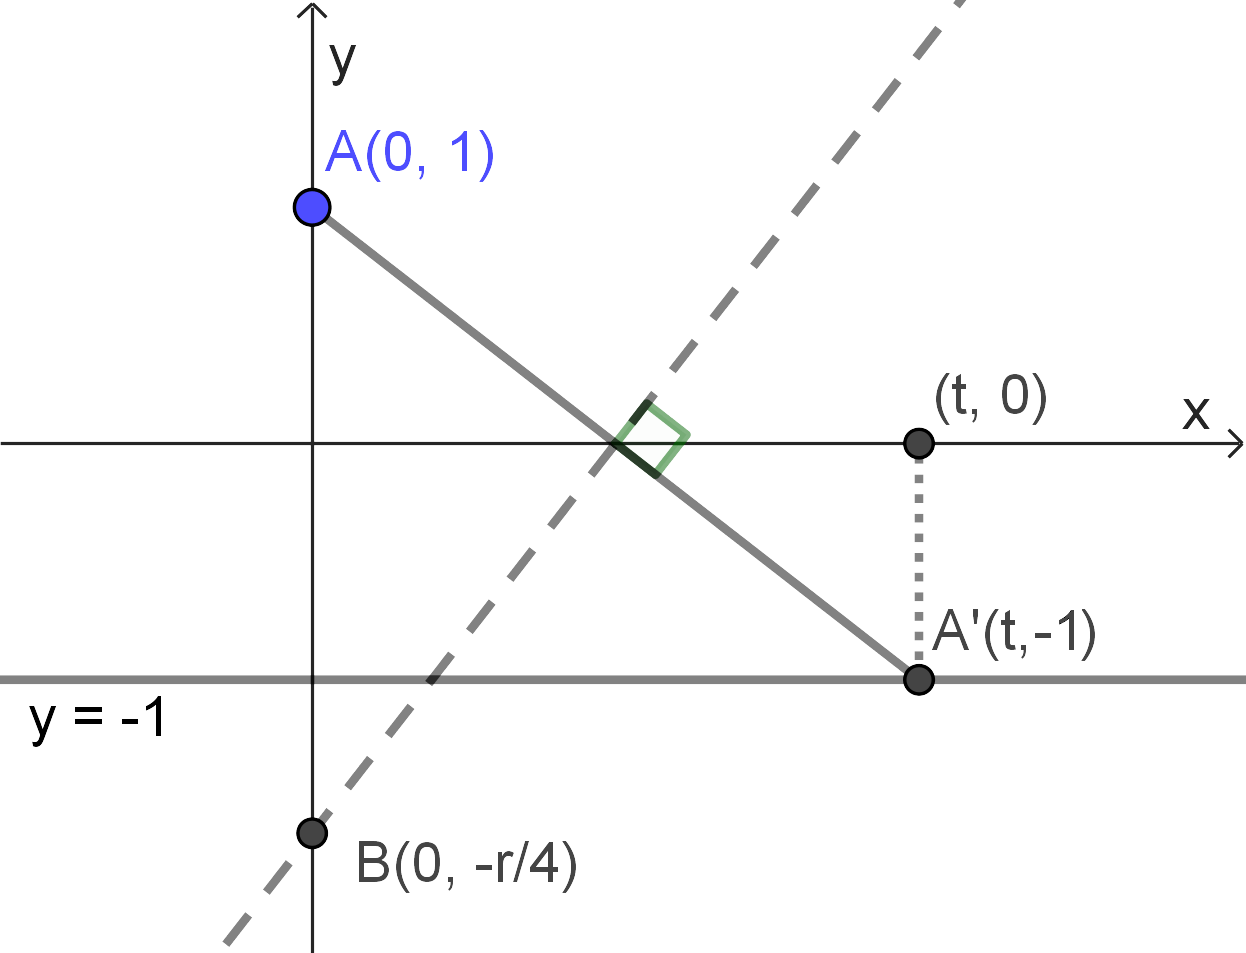
\includegraphics[width=0.4\textwidth]{images/kvadratni_koren.png}
        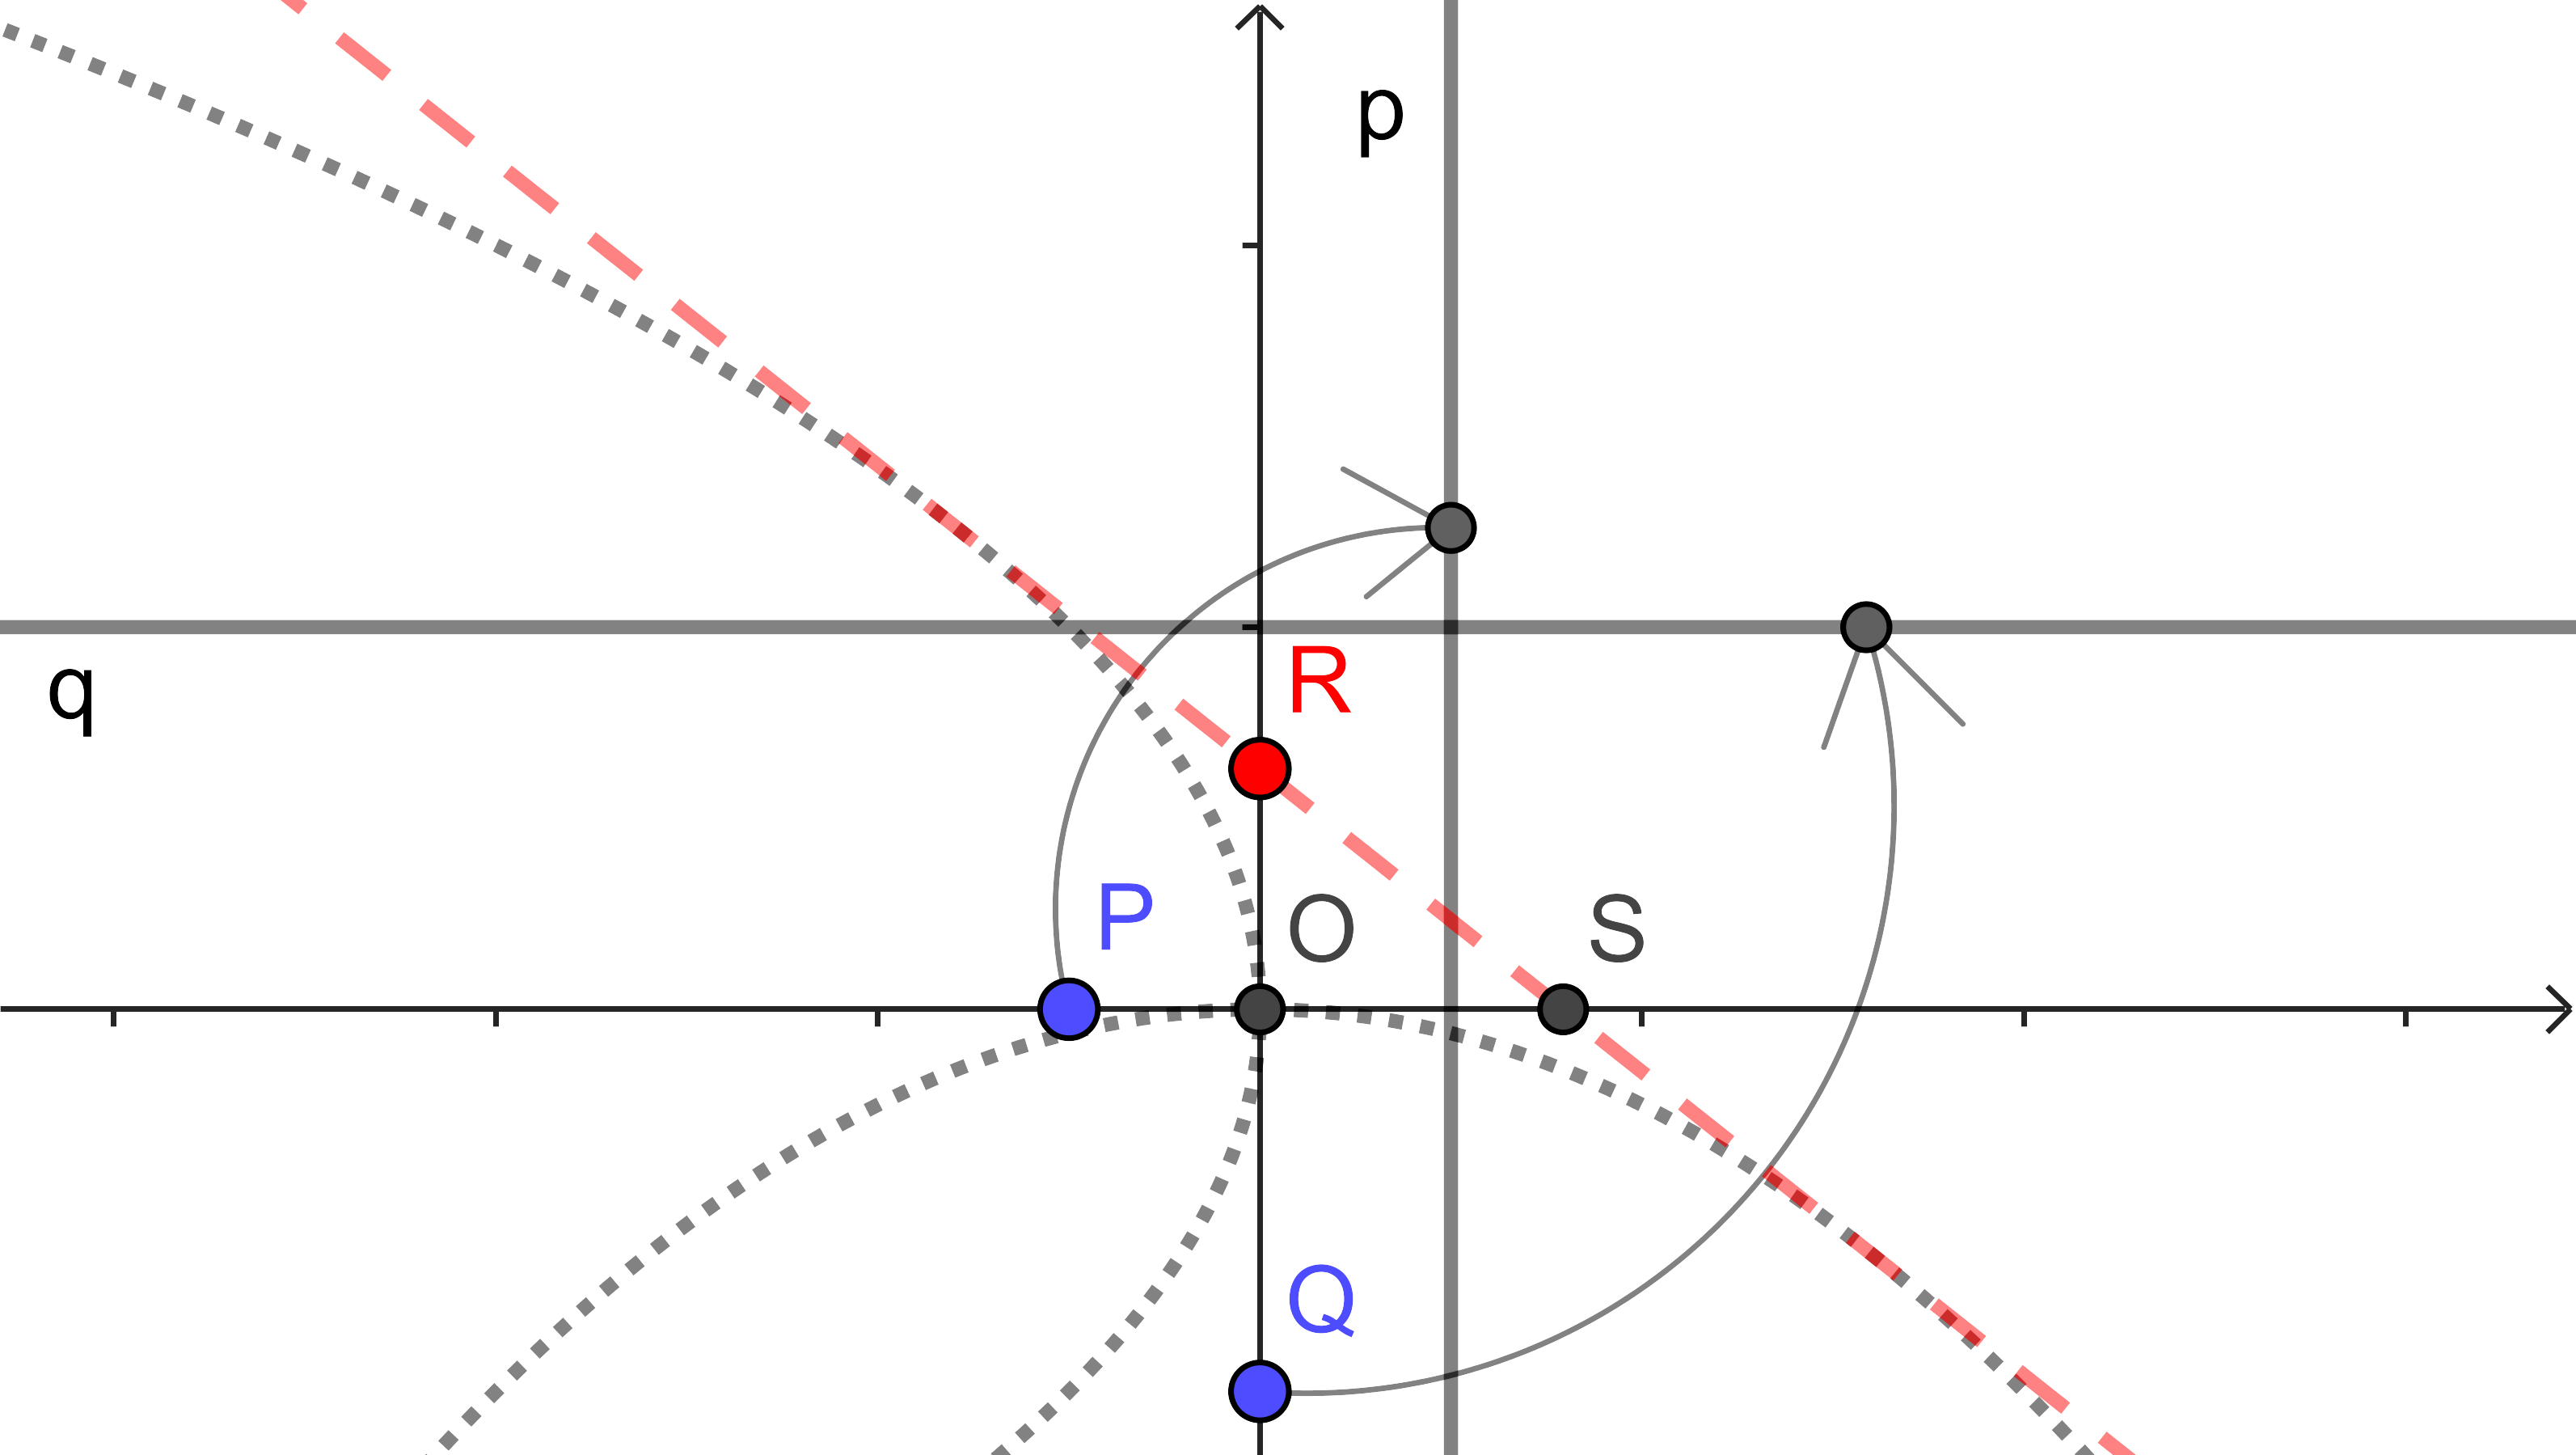
\includegraphics[width=0.5\textwidth]{images/starogr_problemi/cube_martin.png}
    \end{figure}
    \begin{alertblock}{Posledica $2.31$}
        Množica evklidsko-konstruktibilnih števil je prava podmnožica množice $\mathbb{O}$.
    \end{alertblock}
    Origami števila so tista števila, ki jih lahko zapišemo z znaki
    $$ (\;)\;0\;1\;2\;3\;4\;5\;6\;7\;8\;9\;i\;+\;-\;\times\;\div\;\sqrt{\;}\;\sqrt[3]{\;}.$$
\end{frame}

%------------------------------------------------


%------------------------------------------------
\section{Primeri uporabe prepogibanja papirja}
%------------------------------------------------

%------------------------------------------------

\begin{frame}{Konstrukcija pravilnih $n$-kotnikov}
    \begin{alertblock}{Gauss-Wantzlov izrek (izrek $2.38$)}
        Pravilni $n$-kotnik je evklidsko-konstruktibilen natanko takrat, ko je $n = 2^a p_1 \cdots p_k$ za neka $a,k \in \mathbb{N}_0$, kjer so $p_1, \ldots, p_k$ različna Fermatova praštevila, tj.\ $p_i = 2^{2^{m_i}} + 1$ kjer je $m_i \in \mathbb{N}_0$.
    \end{alertblock}
    $$ 3, 4, 5, 6, 8, 10, 12, 15, 16, 17, 20 $$
    \begin{alertblock}{Izrek $2.40$}
        Pravilni $n$-kotnik se lahko konstruira z origamijem natanko takrat, ko je $n = 2^a 3^b p_1 \cdots p_k$ za neke $a,b,k \in \mathbb{N}_0$, kjer so $p_1, \ldots, p_k$ različna Pierpontova praštevila, tj.\ $p_i > 3$ in $p_i = 2^{m_i}3^{n_i} + 1$ za neka $m_i,n_i \in \mathbb{N}_0$.
    \end{alertblock}
    $$ 3, 4, 5, 6, 7, 8, 9, 10, 12, 13, 14, 15, 16, 17, 18, 19, 20 $$
\end{frame}

%------------------------------------------------

\begin{frame}{Konstrukcija pravilnega 7-kotnika}
    \begin{figure}[h]
        \centering
        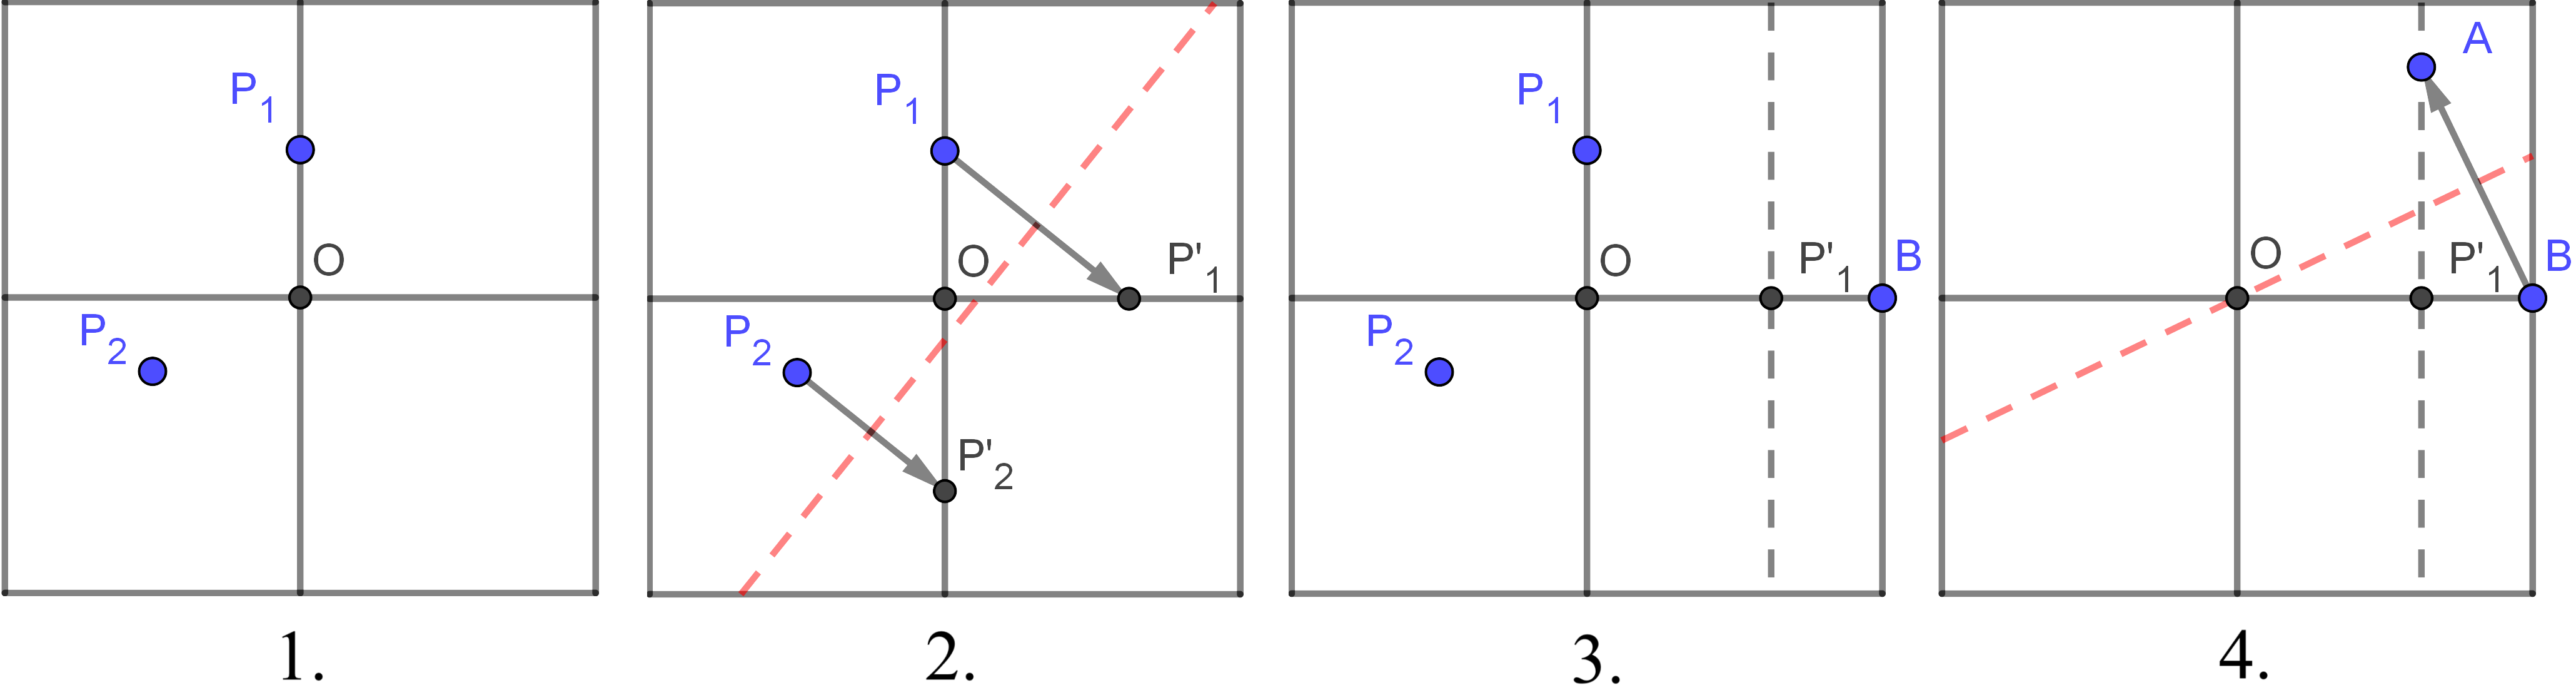
\includegraphics[width=\textwidth]{images/n-kotniki/7kotnik_konstr1.png}
    \end{figure}
    \begin{figure}[h]
        \centering
        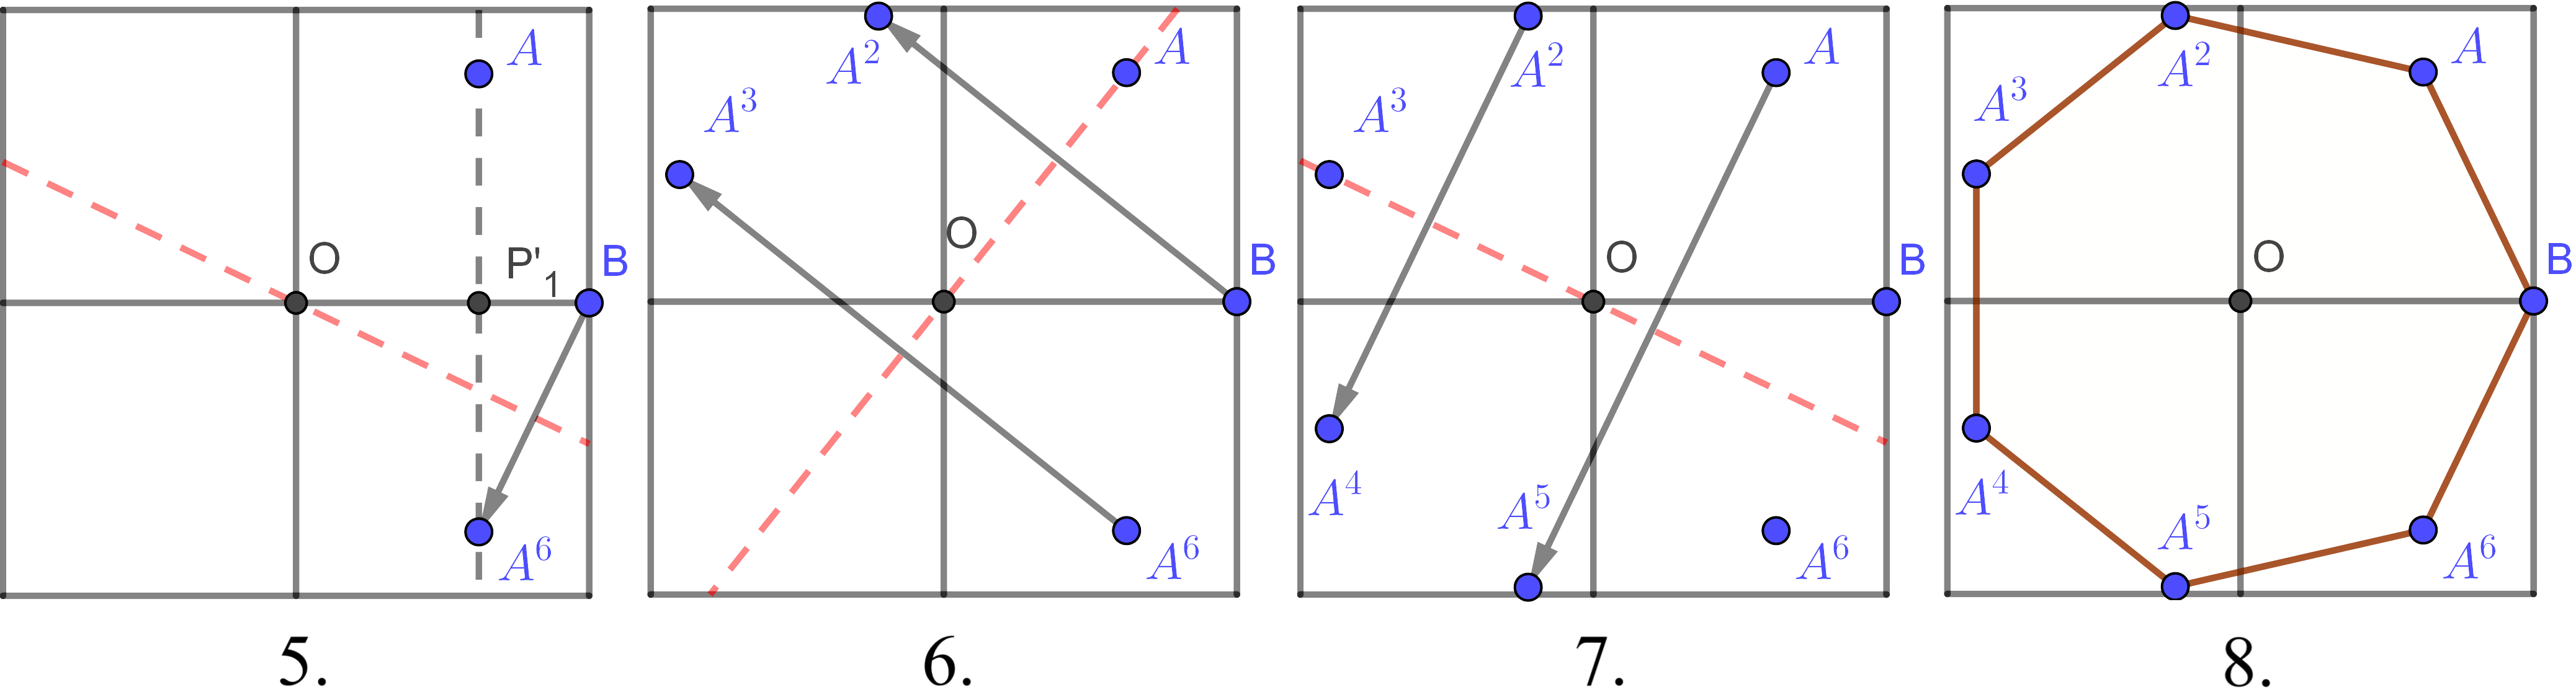
\includegraphics[width=\textwidth]{images/n-kotniki/7kotnik_konstr2.png}
    \end{figure}
\end{frame}

%------------------------------------------------

\begin{frame}{Uporaba v osnovni šoli}
    \begin{figure}[h]
        \centering
        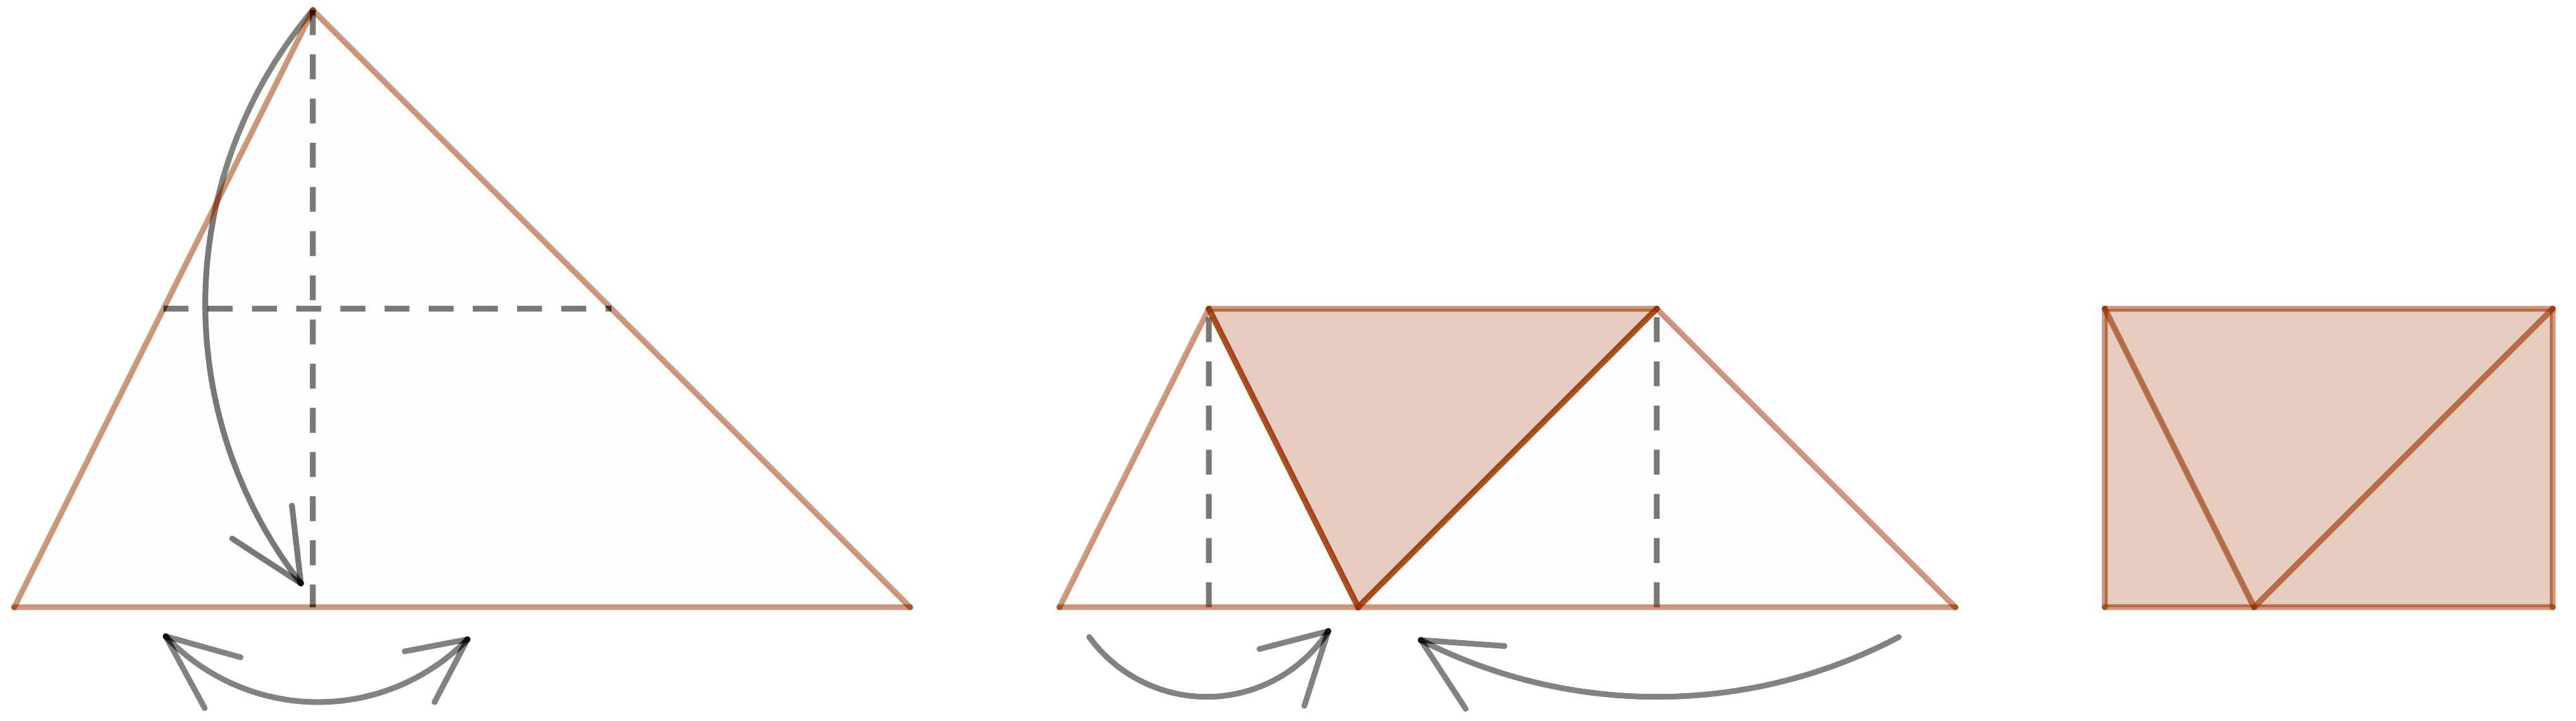
\includegraphics[width=0.7\textwidth]{images/osnovnosolski_prikazi/trikotnik_vsota_kotov.png}
        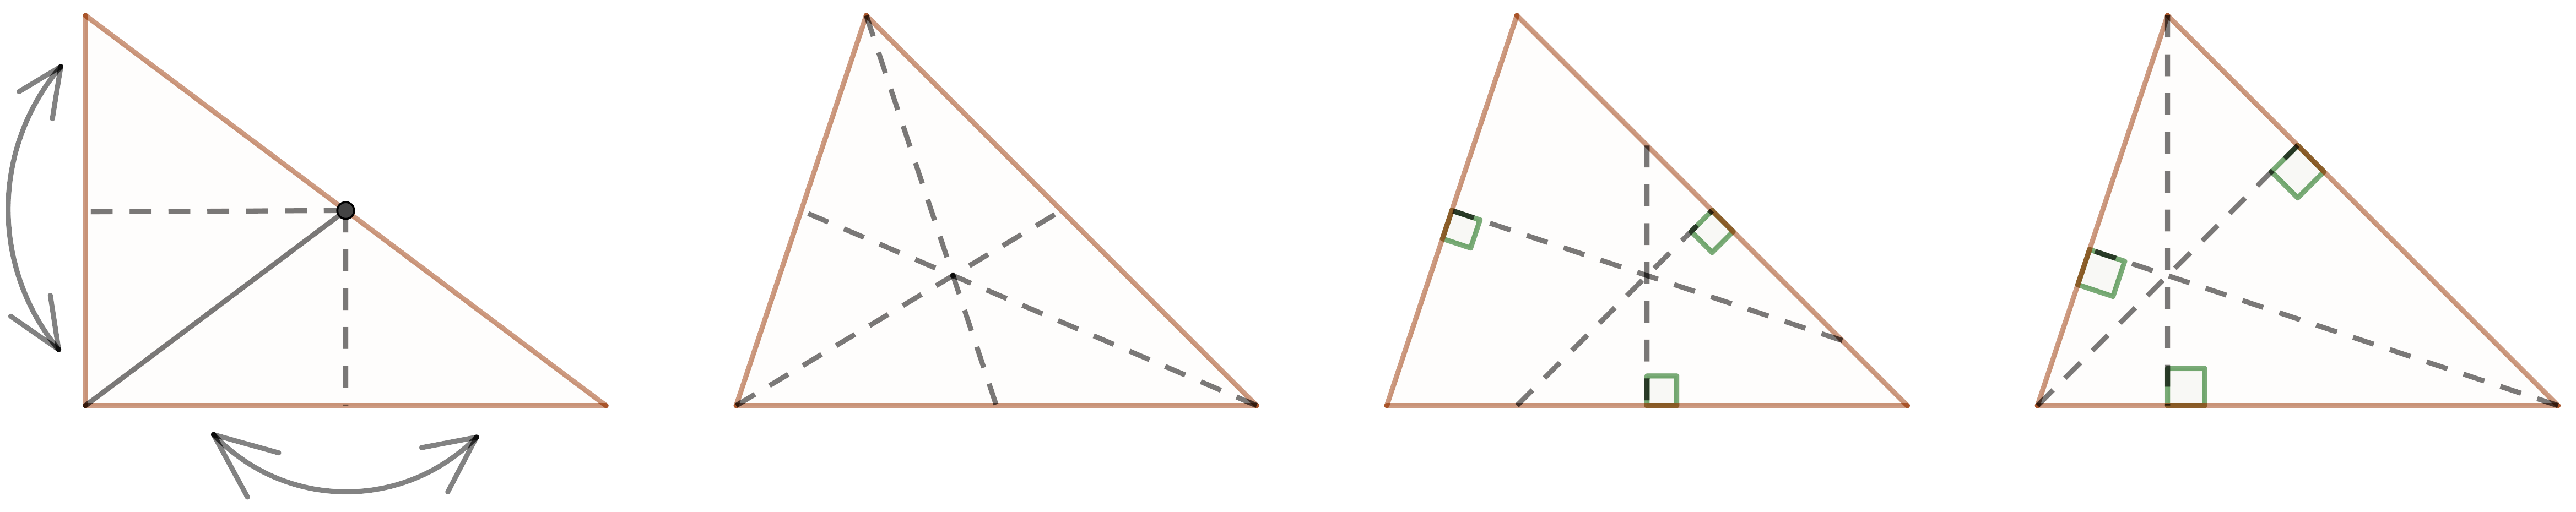
\includegraphics[width=0.9\textwidth]{images/osnovnosolski_prikazi/vec_lastnosti1.png}
        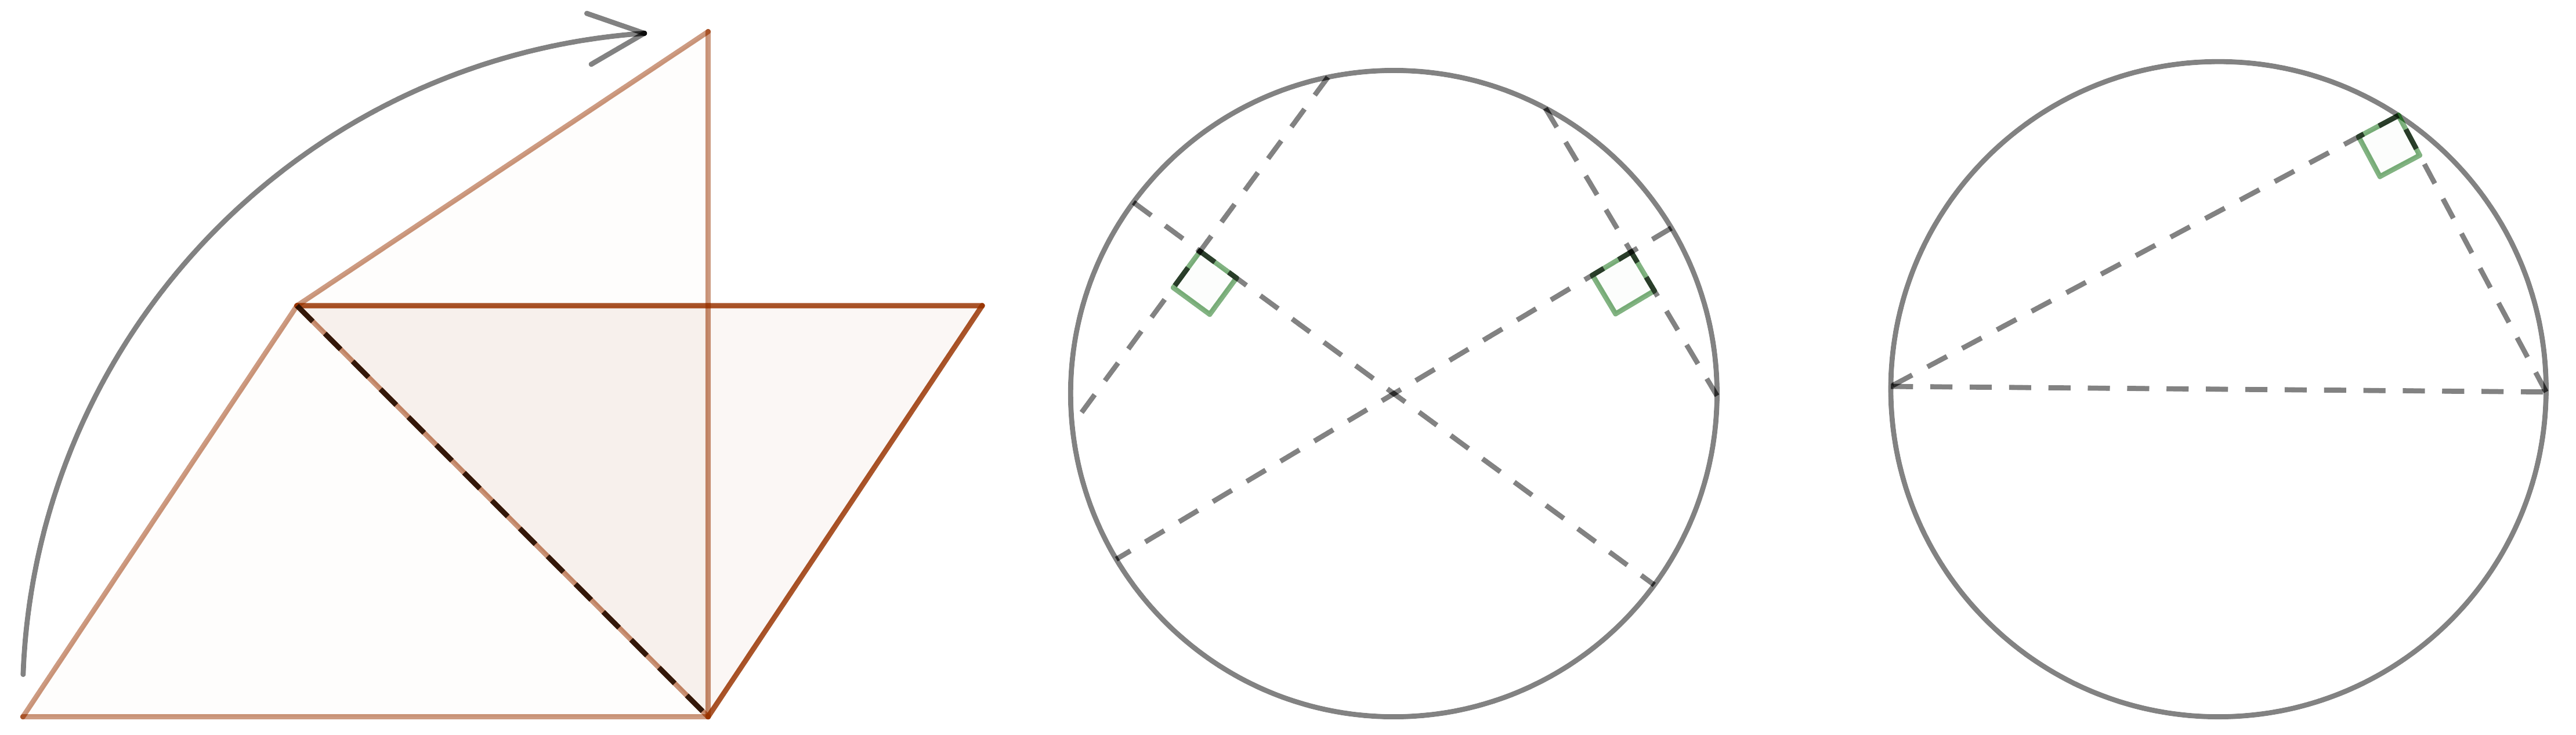
\includegraphics[width=0.8\textwidth]{images/osnovnosolski_prikazi/vec_lastnosti2.png}
    \end{figure}
\end{frame}

%------------------------------------------------

\begin{frame}{Konstrukcije nekaterih pravilnih likov}
    \begin{figure}[h]
        \centering
        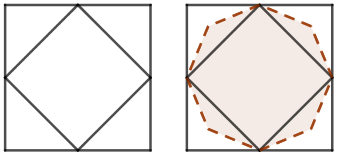
\includegraphics[width=0.5\textwidth]{images/n-kotniki/8kotnik_basic.png}
        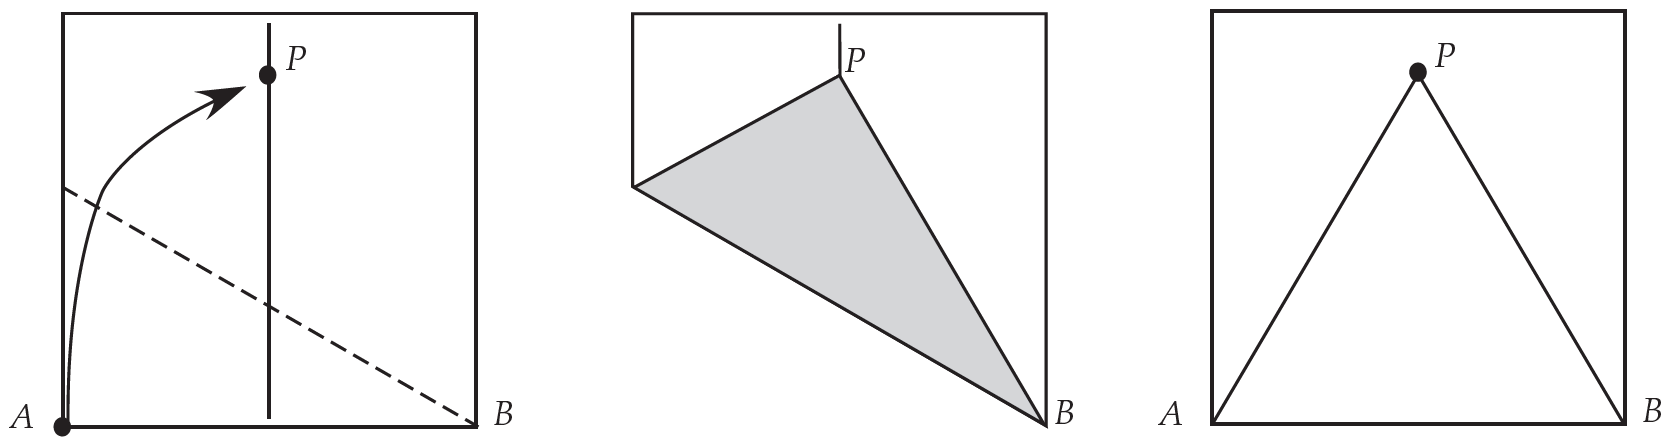
\includegraphics[width=0.8\textwidth]{images/n-kotniki/trik_enak_basic.png}
    \end{figure}
    \begin{figure}[h]
        \centering
        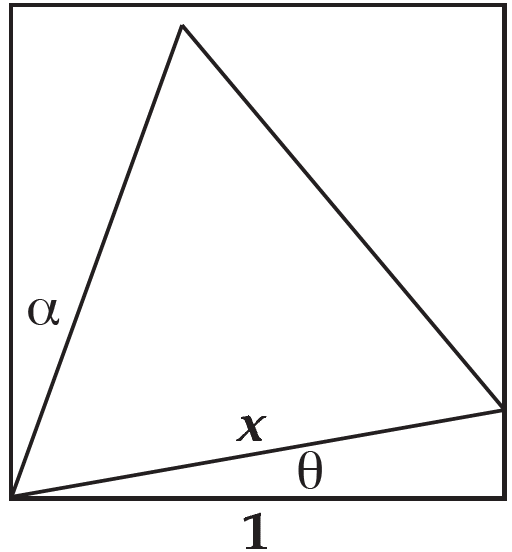
\includegraphics[width=0.2\textwidth]{images/n-kotniki/trik_enak_max1.png}
        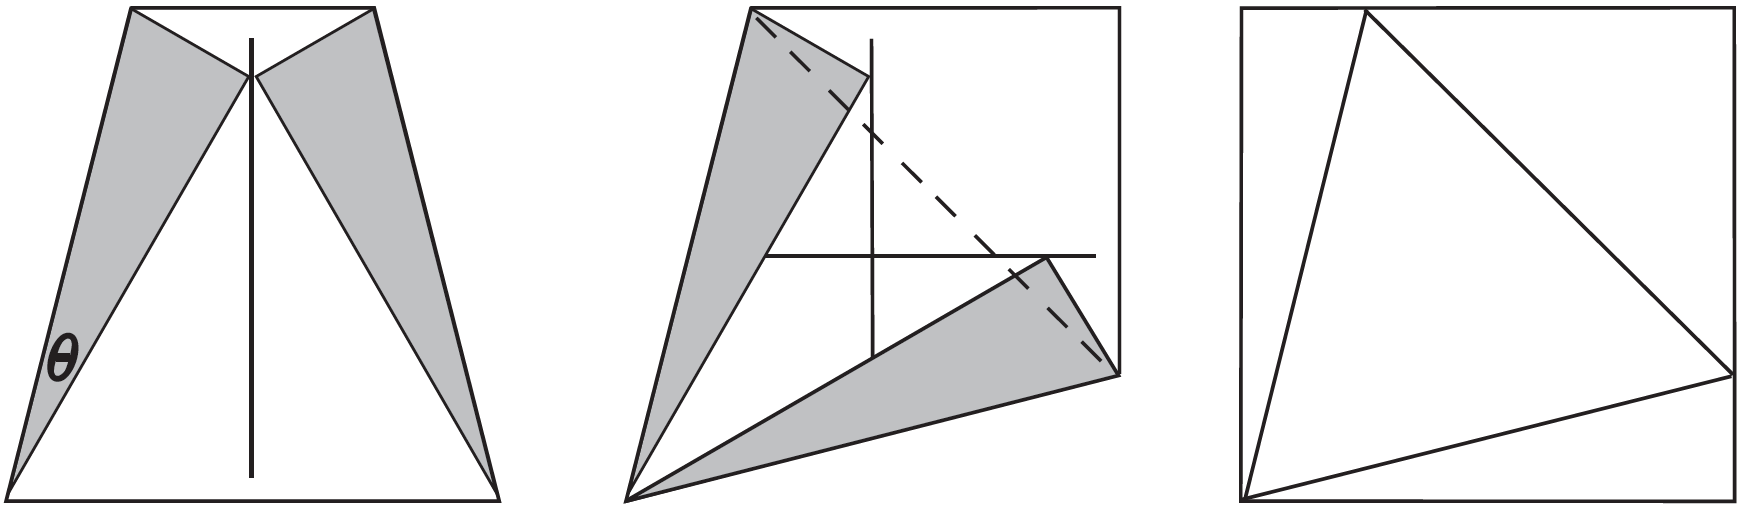
\includegraphics[width=0.7\textwidth]{images/n-kotniki/trik_enak_max2.png}
    \end{figure}
\end{frame}

%------------------------------------------------

\begin{frame}{Prvi, drugi in tretji Hagov izrek}
    \begin{figure}[h]
        \centering
        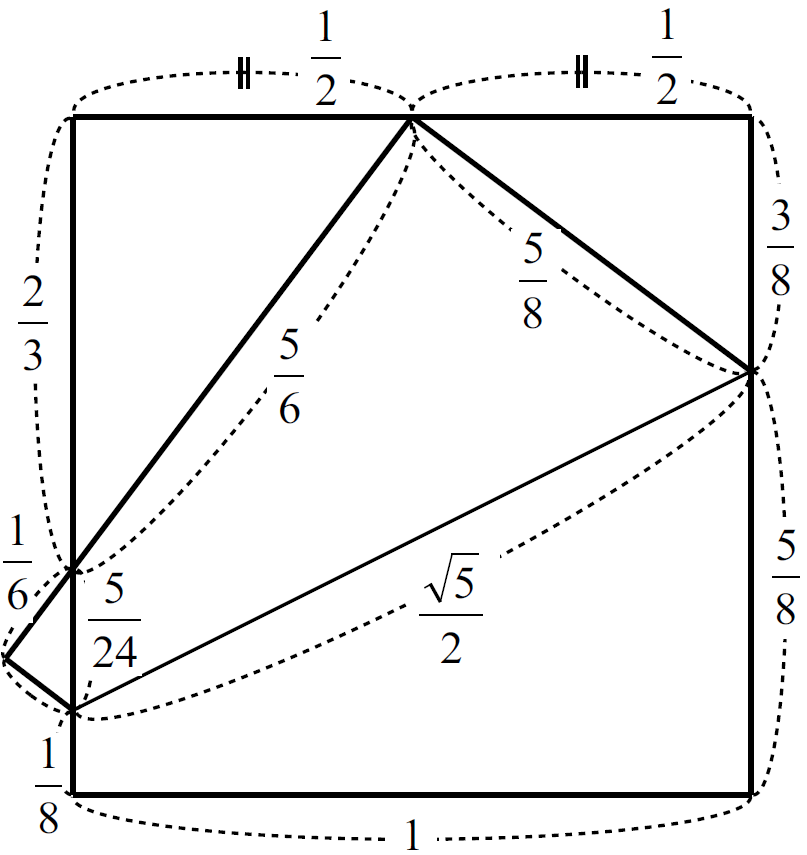
\includegraphics[width=0.32\textwidth]{images/hagovi_izreki/hagov_izrek1_stevilke.png}
        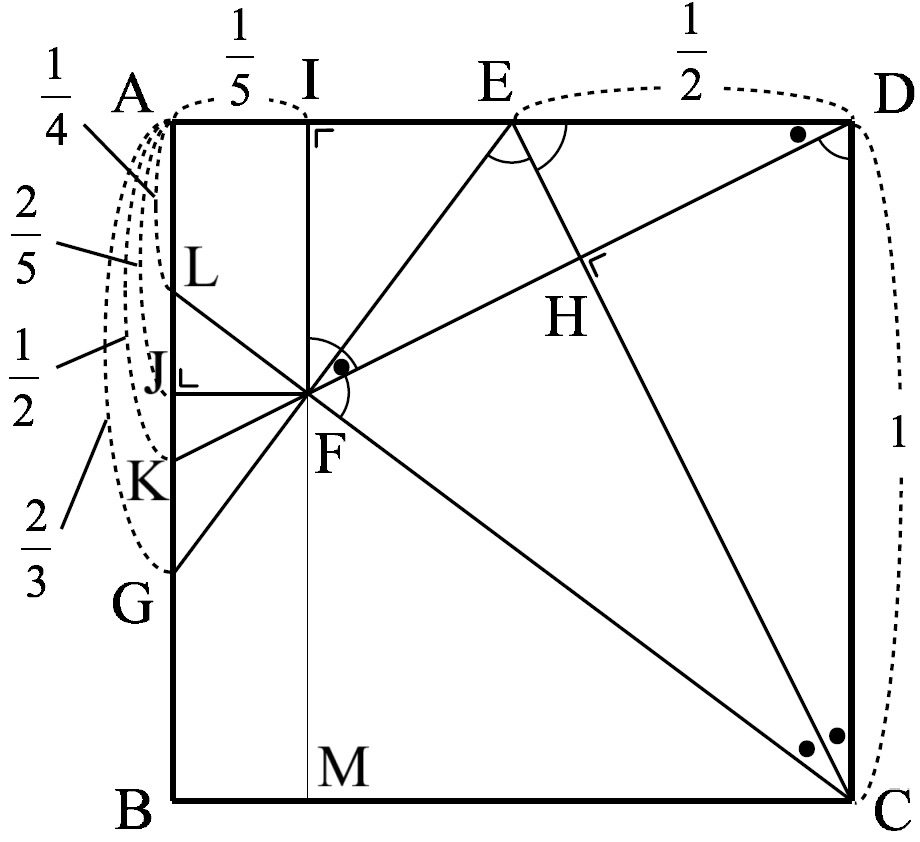
\includegraphics[width=0.35\textwidth]{images/hagovi_izreki/hagov_izrek2_stevilke.png}
        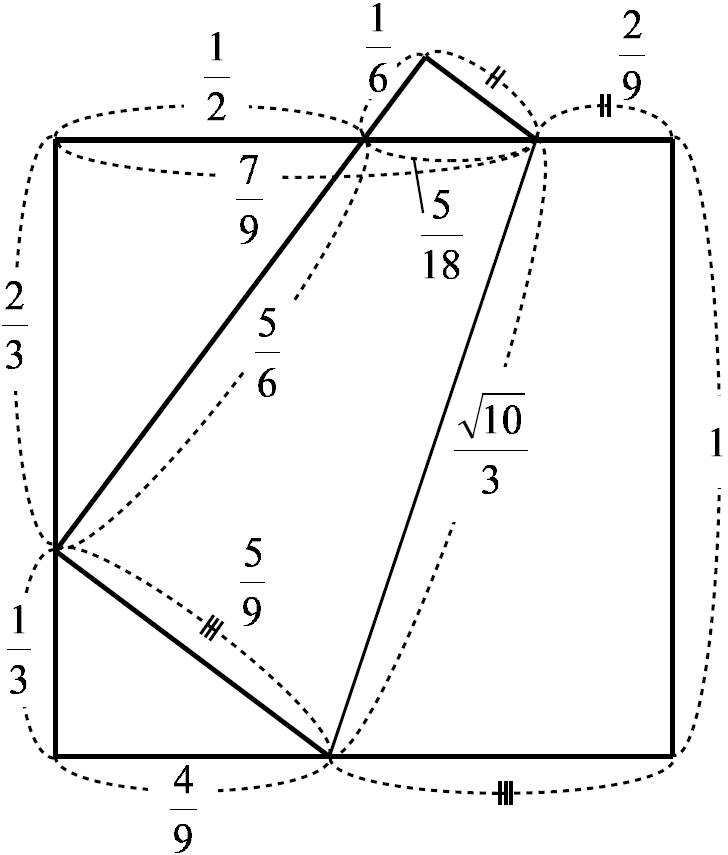
\includegraphics[width=0.3\textwidth]{images/hagovi_izreki/hagov_izrek3_stevilke.png}
    \end{figure}
\end{frame}

%------------------------------------------------

\begin{frame}{Razdelicev daljice na $n$ delov}
    \begin{figure}[h]
        \centering
        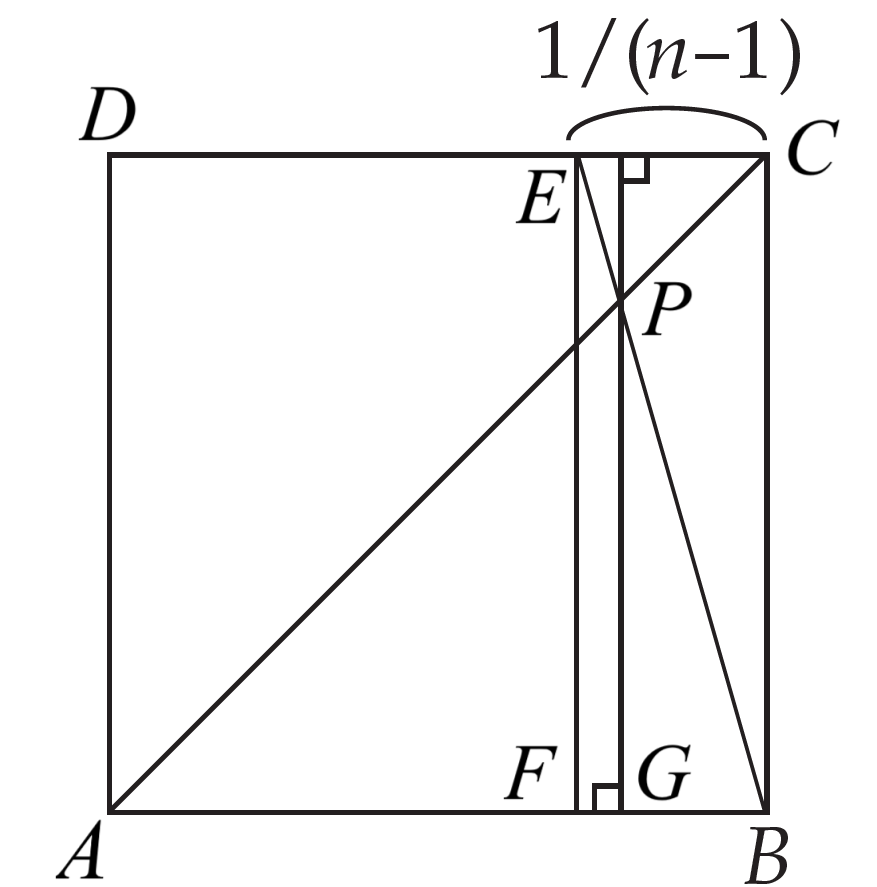
\includegraphics[width=0.3\textwidth]{images/razdelitev_stranice_n1.png}
        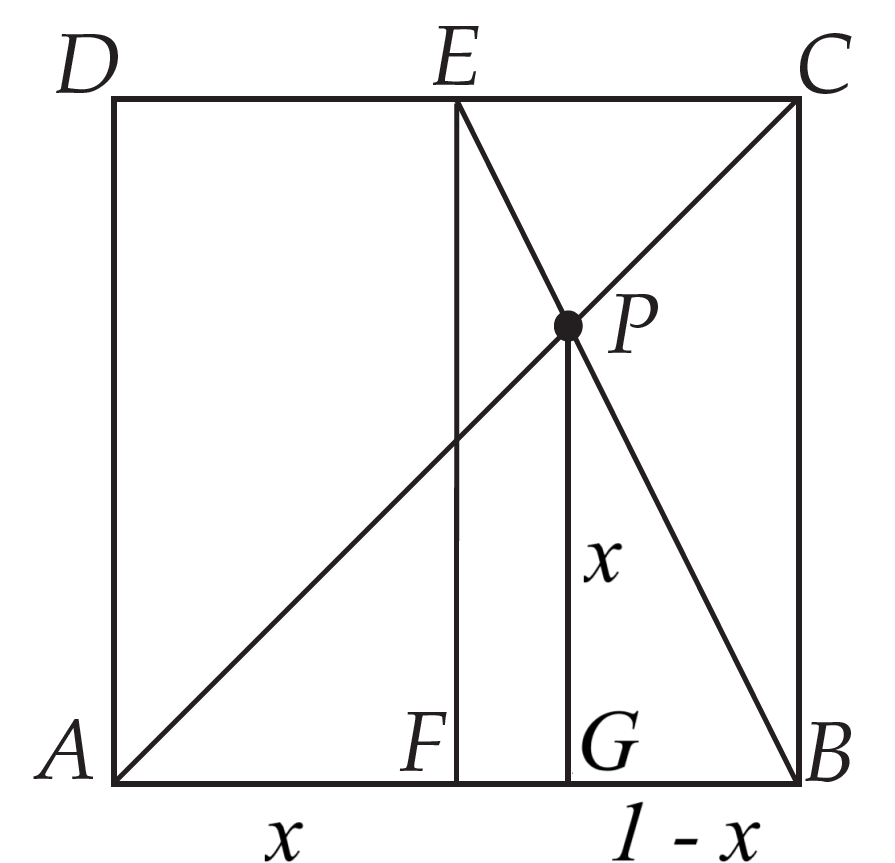
\includegraphics[width=0.3\textwidth]{images/tretjinjenje_stranice2.png}
        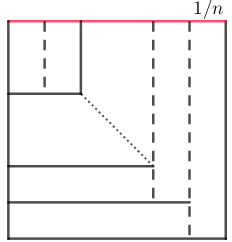
\includegraphics[width=0.3\textwidth]{images/razdelitev_daljice_n1.png}
    \end{figure}
\end{frame}

%------------------------------------------------

\begin{frame}{X-pregibi}
    \begin{figure}[h]
        \centering
        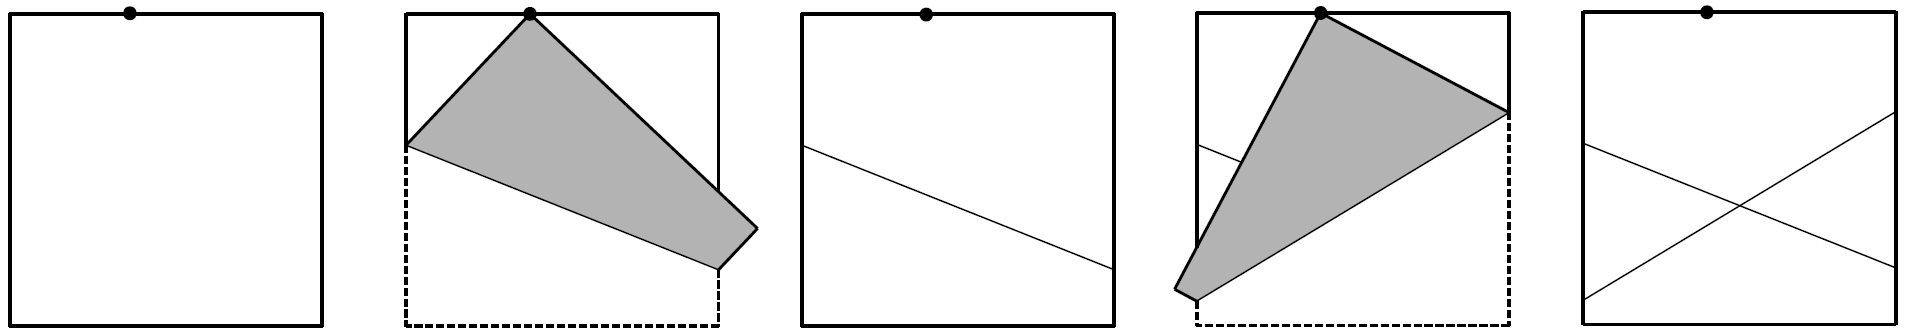
\includegraphics[width=0.85\textwidth]{images/x-pregibi/konstrukcija.png}
        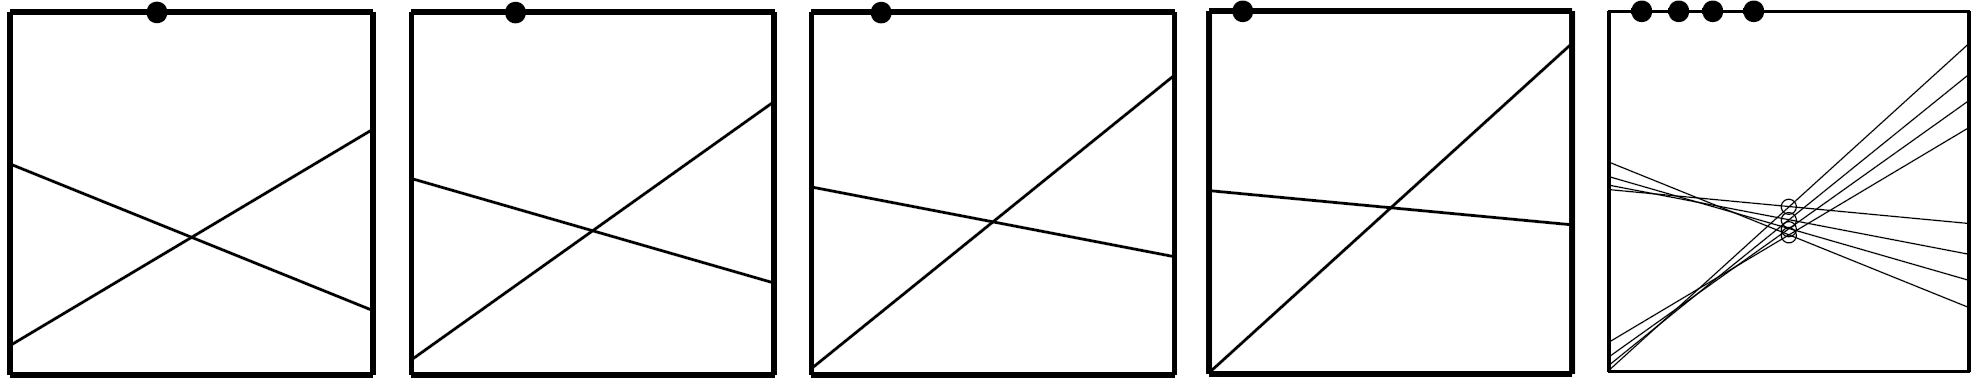
\includegraphics[width=0.9\textwidth]{images/x-pregibi/primeri_skupaj.png}
        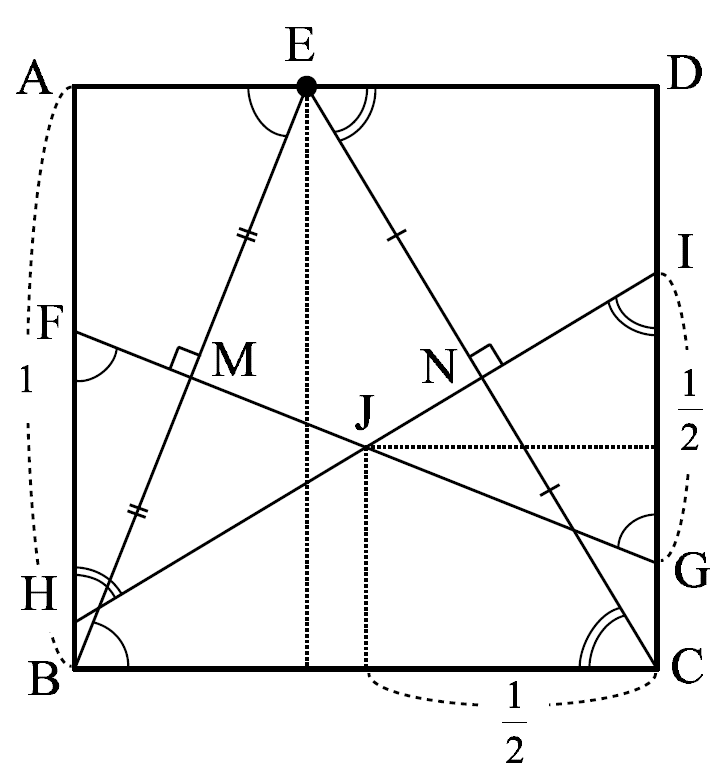
\includegraphics[width=0.35\textwidth]{images/x-pregibi/dokaz_odseki.png}
    \end{figure}
    
\end{frame}

%------------------------------------------------

\begin{frame}{Starogrški problemi}
    \begin{itemize}
        \item \textbf{Podvojitev kocke:} Za dano kocko konstruiraj novo kocko, ki ima dvakrat večji volumen od prve (konstrukcija razdalje $\sqrt[3]{2}$).
        \item \textbf{Trisekcija kota:} Za dan kot $\alpha$ konsturiraj kot $\alpha/3$.
        \item \textbf{Kvadratura kroga:} Za dan krog konstruiraj kvadrat, ki ima enako ploščino kot dani krog (konstrukcija razdalje $\sqrt{\pi}$).
    \end{itemize}
\end{frame}

%------------------------------------------------

\begin{frame}{Podvojitev kocke -- Martinova in Messerjeva konstrukcija}
    \begin{figure}[h]
        \centering
        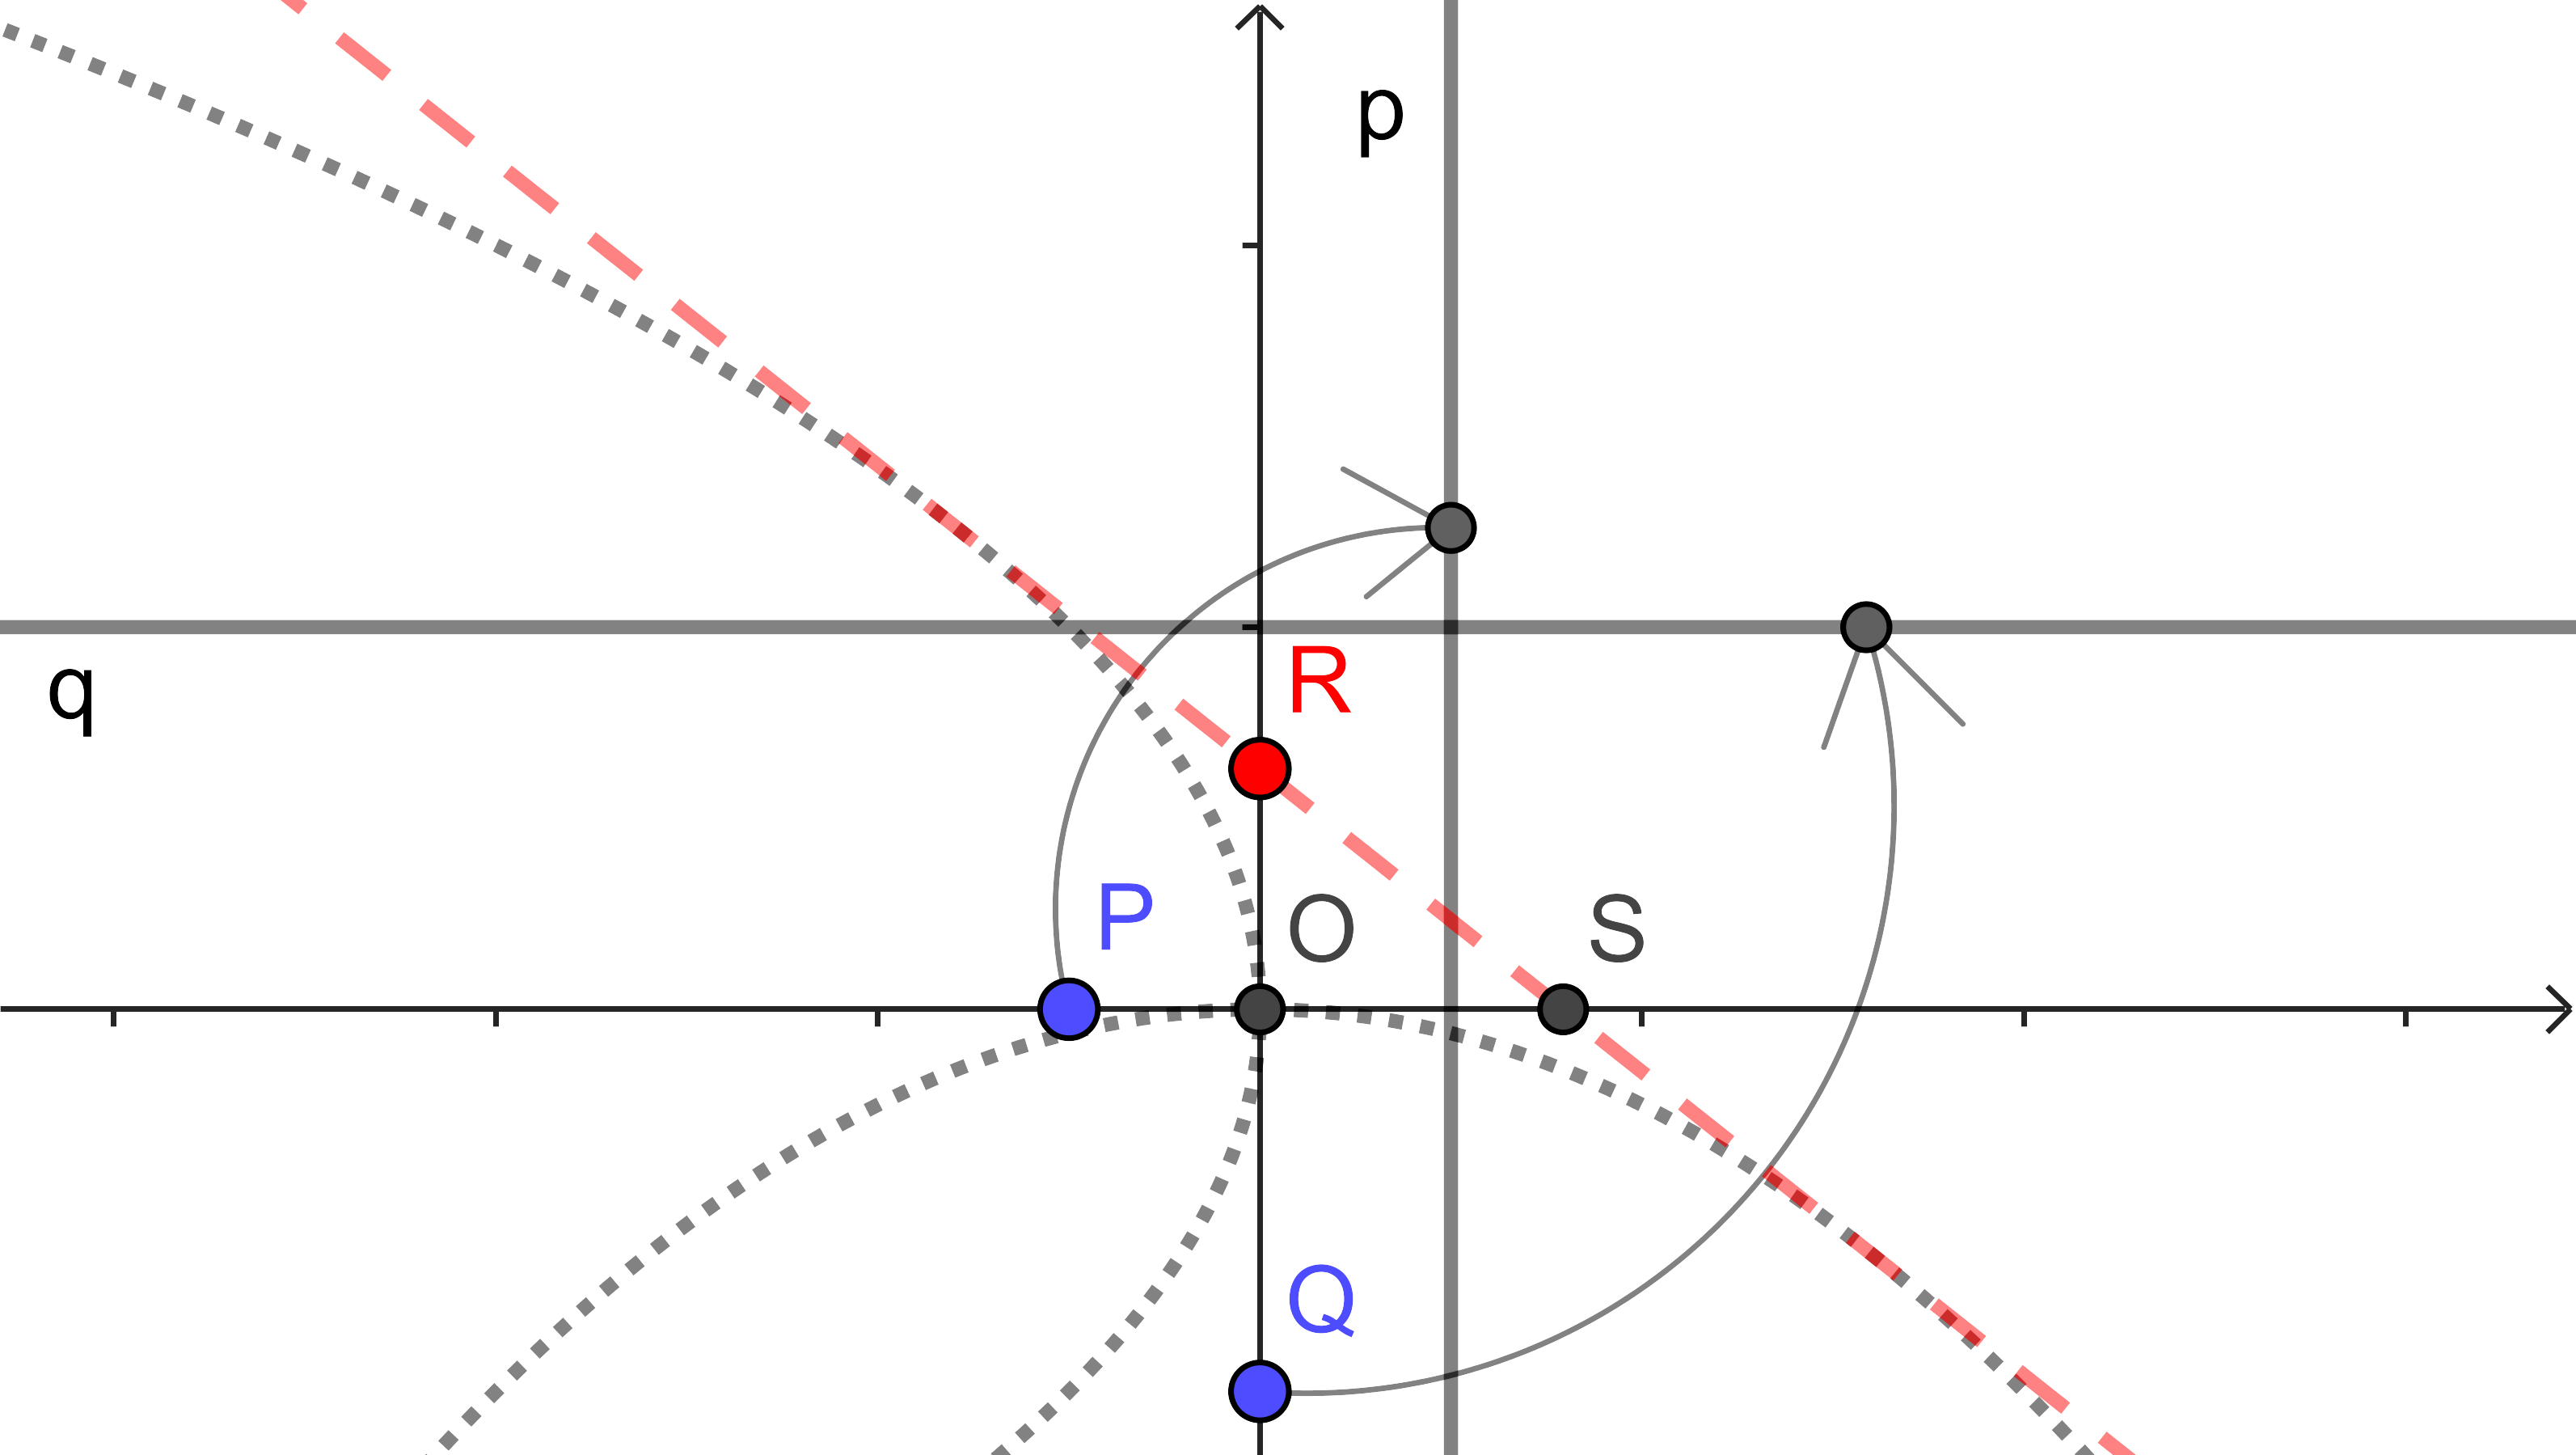
\includegraphics[width=0.5\textwidth]{images/starogr_problemi/cube_martin.png}
    \end{figure}
    \begin{figure}[h]
        \centering
        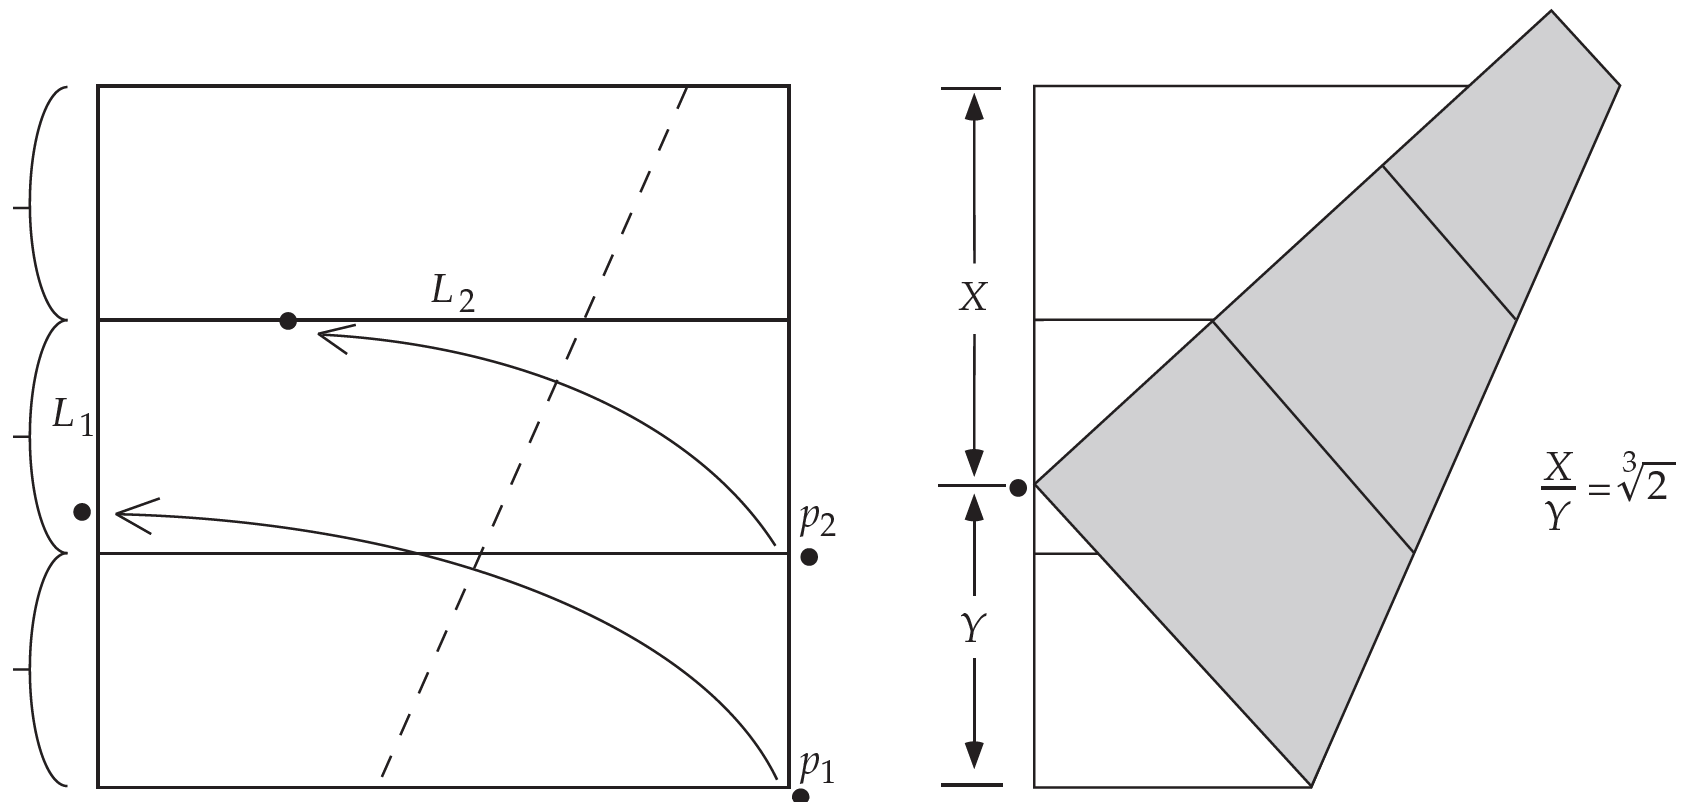
\includegraphics[width=0.68\textwidth]{images/starogr_problemi/messer1.png}
        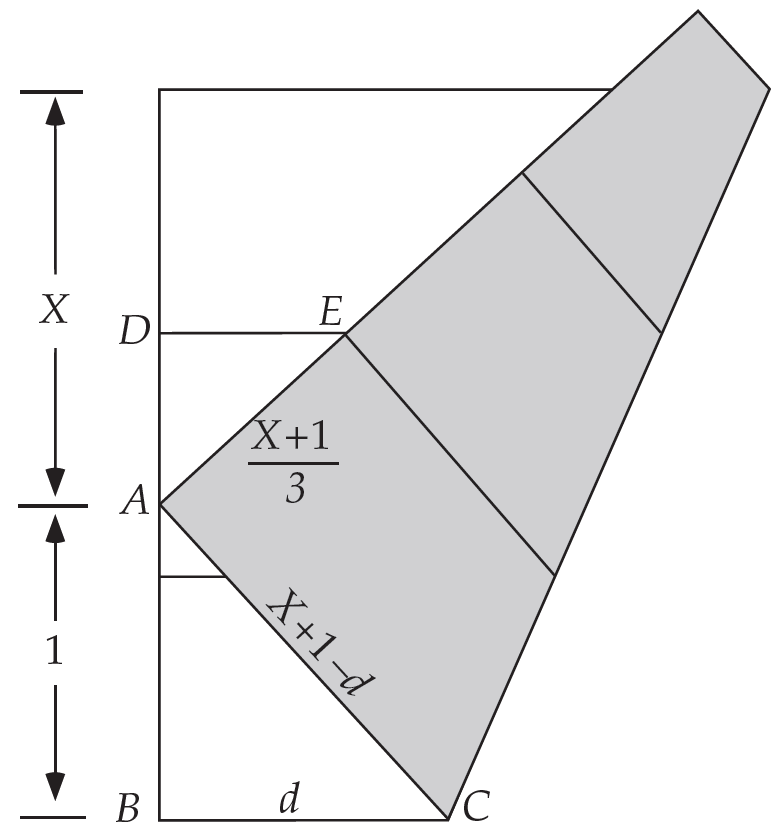
\includegraphics[width=0.3\textwidth]{images/starogr_problemi/messer2.png}  
    \end{figure} 
\end{frame}

%------------------------------------------------

\begin{frame}{Trisekcija kota -- Abejeva in Justinova metoda}
    \begin{figure}[h]
        \centering
        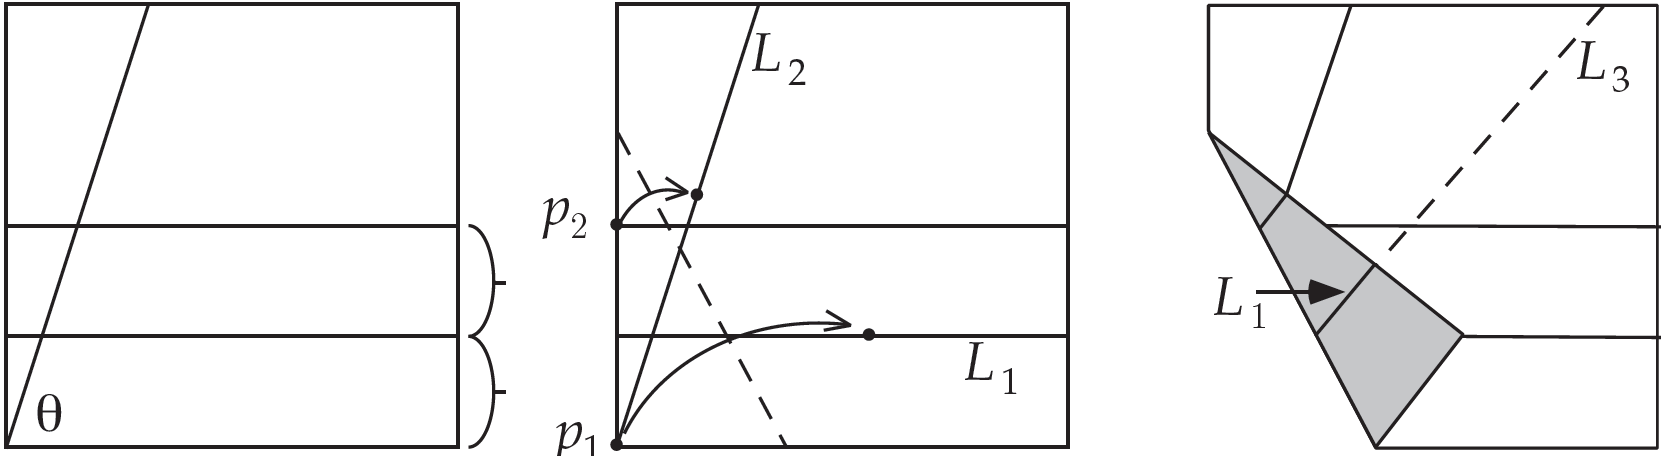
\includegraphics[width=0.8\textwidth]{images/starogr_problemi/abe_nastavek1.png}
        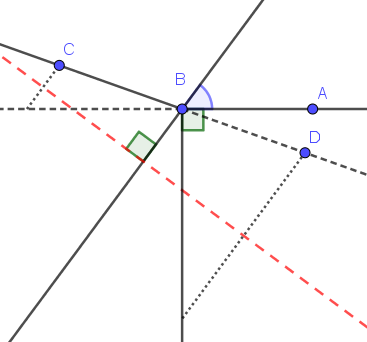
\includegraphics[width=0.4\textwidth]{images/starogr_problemi/justin_trisection.png}
        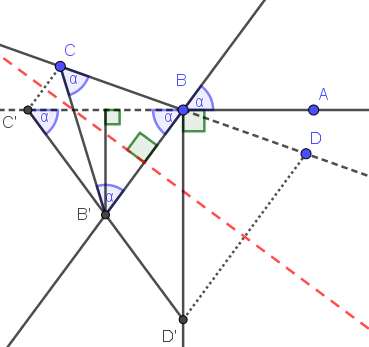
\includegraphics[width=0.4\textwidth]{images/starogr_problemi/justin_trisection_dokaz.png}    
    \end{figure}
\end{frame}
%------------------------------------------------

\begin{frame}{Tangente na stožnice}
    \begin{figure}[h]
        \centering
        
\includegraphics[width=0.2\textwidth]{images/stožnice/folding_parabola_1.png}
        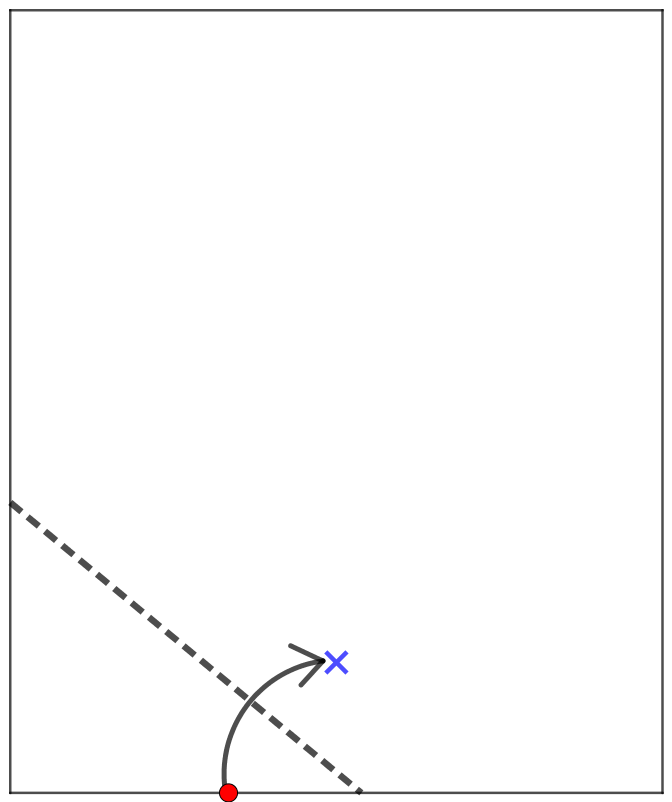
\includegraphics[width=0.2\textwidth]{images/stožnice/folding_parabola_2.png}
        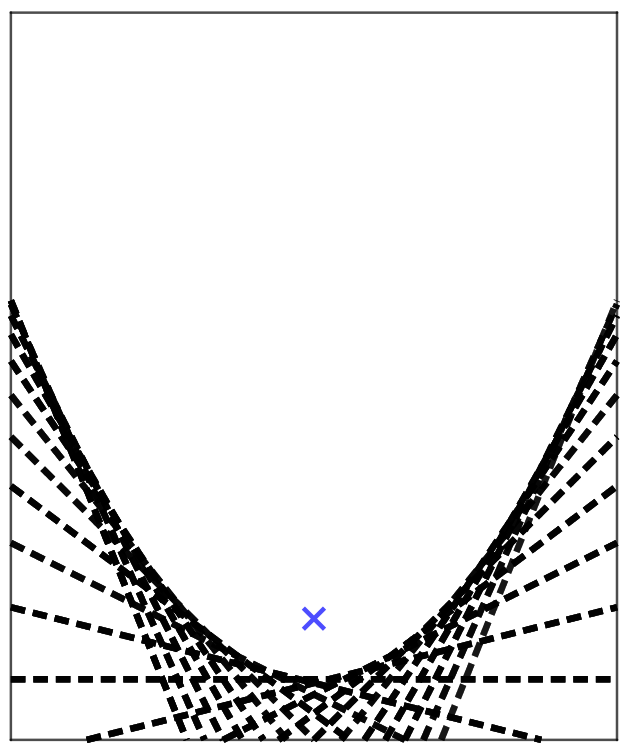
\includegraphics[width=0.2\textwidth]{images/stožnice/folding_parabola_3.png}
    \end{figure}
    \begin{figure}[h]
        \centering
        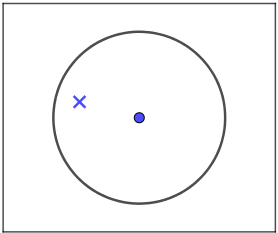
\includegraphics[width=0.3\textwidth]{images/stožnice/folding_elipsa_1.png}
        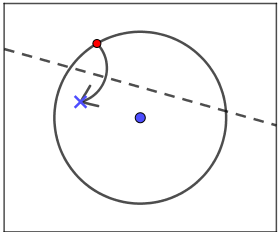
\includegraphics[width=0.3\textwidth]{images/stožnice/folding_elipsa_2.png}
        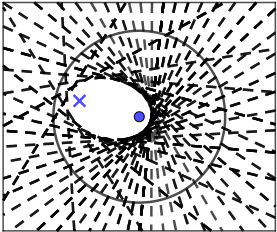
\includegraphics[width=0.3\textwidth]{images/stožnice/folding_elipsa_3.png}
    \end{figure}    
\end{frame}

%------------------------------------------------

%------------------------------------------------
\section{Reševanje enačb}
%------------------------------------------------

\begin{frame}{Lillova metoda}
    Iščemo realne ničle polinoma
    $$ p(x) = a_n x^n + a_{n-1} x^{n-1} + \ldots + a_2 x^2 + a_1 x + a_0. $$
    \begin{figure}[h]
        \centering
        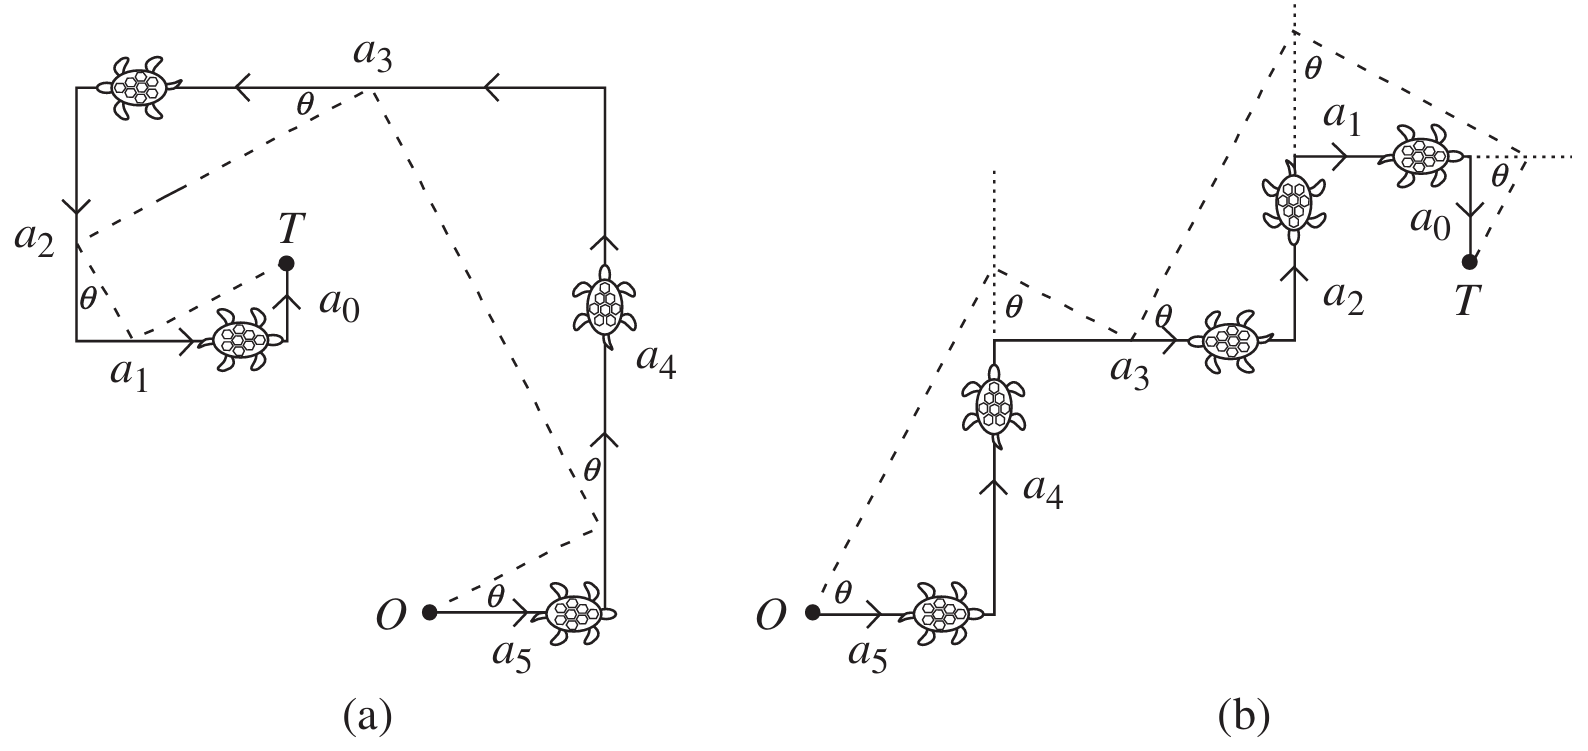
\includegraphics[width=0.9\textwidth]{images/kubična enačba/primera_zelvine_poti.png}
    \end{figure}
    \begin{alertblock}{Trditev 6.1}
        Število $x_{\theta} = - \tan \theta$ je ničla polinoma $p$.
    \end{alertblock}
\end{frame}

%------------------------------------------------

\begin{frame}{Belochin postopek za reševanje kubične enačbe}
    \begin{columns}
        \begin{column}{0.6\textwidth}
            $$ax^3 + bx^2 + cx + d = 0$$
            \begin{enumerate}
                \item Po koeficientih narišemo želvino pot iz točke $A(0,0)$ v točko $B$.
                \item Zarišemo premice $r: x=a, s: y=b, r': x=2a$ in $s':y=b+d$.
                \item Z Belochinim pregibom točko $A$ položimo na premico $r'$ in točko $B$ na premico $s'$.
                \item Izmerimo kot z vrhom v točki $A$.
            \end{enumerate}
            Primer: $x^3 - 6x^2 + 11x - 6 = 0$
         \end{column}
         \begin{column}{0.4\textwidth}
            \begin{figure}[h]
                \centering
                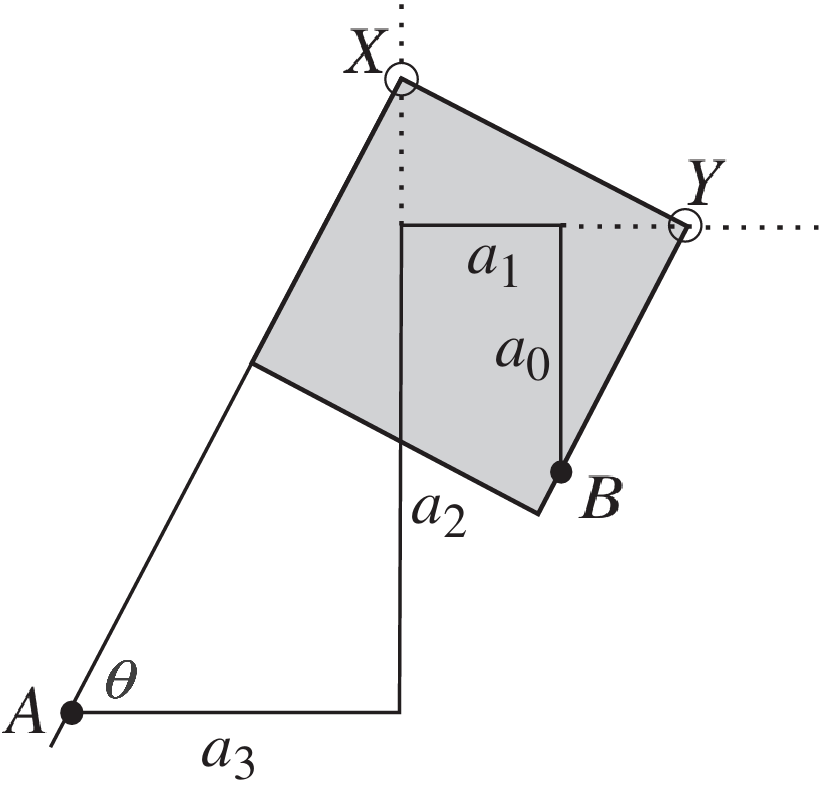
\includegraphics[width=\textwidth]{images/kubična enačba/beloch_kubicna_resitev.png}
            \end{figure}
        \end{column}
    \end{columns}
\end{frame}

%------------------------------------------------

\begin{frame}{Skupne tangente na stožnice}
    Stožnica $\mathcal{S}$ v $P(\mathbb{R}^3)$:
    \begin{equation*}
        \label{eq:stoznica_matricna}
        \mathcal{S}: v^\intercal M v = 0,
        \text{ kjer sta } v =
        \begin{bmatrix}
            x\\
            y\\
            z
        \end{bmatrix}
        \text{ in } M =
        \begin{bmatrix}
            a_{11} & a_{12} & a_{13}\\
            a_{12} & a_{22} & a_{23}\\
            a_{13} & a_{23} & a_{33}
        \end{bmatrix}.
    \end{equation*}
    Tangenta na stožnico $\mathcal{S}$ v točki $V \in \mathcal{S}: p_V$

    Dualna preslikava: $V \mapsto Mv$, kjer je $v \in V$.
    \begin{figure}[h]
        \centering
        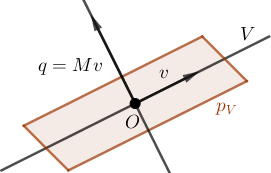
\includegraphics[width=0.4\textwidth]{images/proj_tangenta.png}
    \end{figure}
    Dualna stožnica $\mathcal{S}^*$: množica dualov tangent na $\mathcal{S}$. Njena matrika je $M^{-1}$.
\end{frame}

%------------------------------------------------

\begin{frame}{Skupne tangente na stožnice}
    \begin{alertblock}{}
        Naj bosta $\mathcal{S}_1$ in $\mathcal{S}_2$ stožnici s pripadajočima simetričnima obrnljivima matrikama $M_1$ in $M_2$. Potem je dual skupne tangente skupna točka njunih dualnih stožnic $\mathcal{S}^*_1$ in $\mathcal{S}^*_2$. Torej iščemo $q \in \mathcal{S}^*_1 \cap \mathcal{S}^*_2$, ki reši sistem enačb
        $$ q^\intercal M^{-1}_1 q = 0 \; \text{ in } \; q^\intercal M^{-1}_2 q = 0.$$
    \end{alertblock}
    V praksi: Stožnice v $\mathbb{R^2}$ homogeniziramo v stožnice v $P(\mathbb{R}^3)$, poiščemo skupne tangente in jih dehomoniziramo (afina ravnina: $z=1$).
\end{frame}

%------------------------------------------------

\begin{frame}{Reševanje kubične enačbe}
    $$ x^3 + bx^2 + cx + d = 0, d \neq 0$$

    \begin{itemize}
        \item $\mathcal{P}_1: (y+c)^2 = -4d(x-b)$ z goriščem $F_1 (b - d, -c)$ in premico vodnico $L_1: x = b + d$,
        \item $\mathcal{P}_2: x^2 = -4y$ z goriščem $F_2 (0, -1)$ in premico vodnico $L_2: y = 1$.
    \end{itemize}
    Skupna tangenta: $Ax + By + Cz = 0$.

    Izračunamo $M_1^{-1}$ in $M_2^{-2}$ in za $q = [A:B:C] \in \mathcal{P^*}_1 \cap \mathcal{P^*}_2$ rešujemo sistem $q^\intercal M^{-1}_1 q = 0 \; \text{ in } \; q^\intercal M^{-1}_2 q = 0$. Dobimo
    $$ bA^2 - cAB + AC + dB^2 = 0 \; \text{ in } \; -BC = A^2.$$
    Upoštevamo $z=1$ in nastavimo $B=-1$. Tangenta ima sedaj enačbo $y = Ax + C$. Dobimo $A^3 + bA^2 + cA + d = 0$.

    Primer: $x^3 - 2x^2 - x + 2 = 0$
\end{frame}

%------------------------------------------------

\begin{frame}{Reševanje kvartične enačbe}
    $$ x^4 + bx^2 + 2cx + d = 0, d \neq 0 $$

    \begin{itemize}
        \item krožnica $\mathcal{C}: x^2 + y^2 = r^2$ s središčem v $S(0,0)$ in polmerom $r$ ter
        \item parabola $\mathcal{P}: c^2x^2 - 2cdexy + d^2e^2y^2 - 4d^2ex = 0$.
    \end{itemize}
    Skupna tangenta: $Ax + By + Cz = 0$.

    Izračunamo $M_1^{-1}$ in $M_2^{-2}$ in za $q = [A:B:C] \in \mathcal{P^*}_1 \cap \mathcal{P^*}_2$ rešujemo sistem $q^\intercal M^{-1}_1 q = 0 \; \text{ in } \; q^\intercal M^{-1}_2 q = 0$. Dobimo
    $$ A^2 + B^2 = \frac{C^2}{r^2} \; \text{ in } \; deAC - dB^2 + cBC = 0.$$
    Upoštevamo $z=1$ in nastavimo $B=-1$. Tangenta ima sedaj enačbo $y = Ax + C$. Dobimo $$C^4 + bC^2 + 2cC + d = 0.$$
\end{frame}

%------------------------------------------------

\begin{frame}{Primer}
    $$ 64x^4 - 177x^2 + 143x - 30 = 0 \; \text{ oz. } \; \left(x - \frac{3}{8}\right) \left(x - \frac{5}{8}\right) (x-1) (x+2) = 0.$$
    \begin{figure}[h]
        \centering
        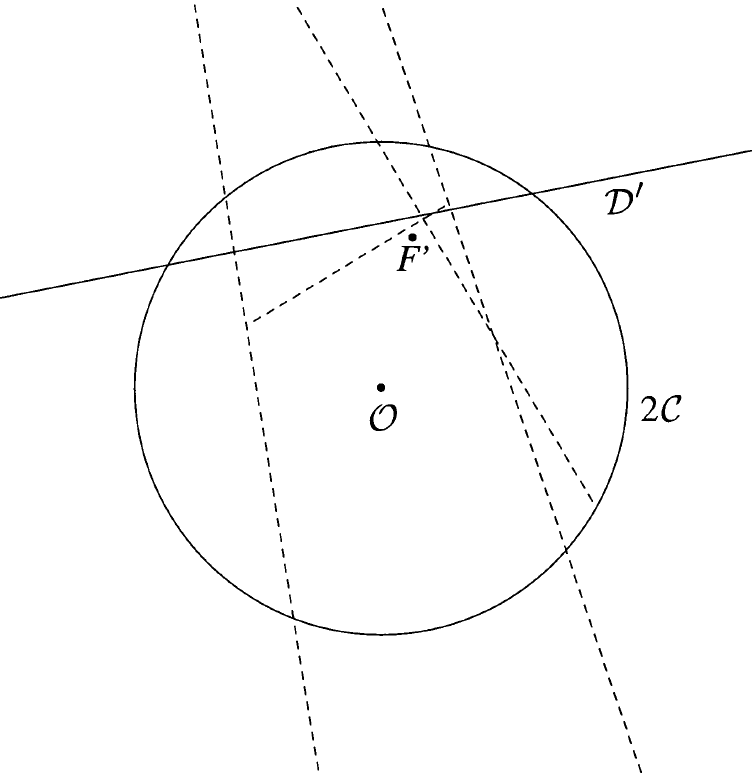
\includegraphics[width=0.35\textwidth]{images/tang_krozn_par1.png}
        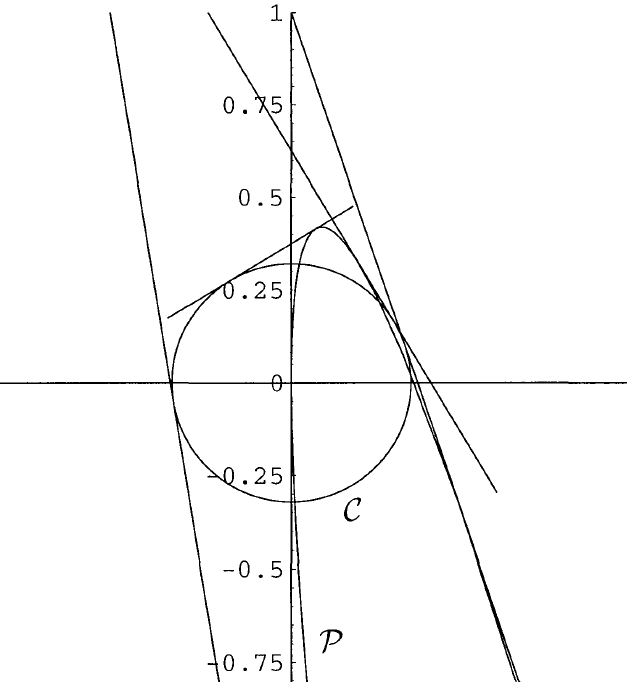
\includegraphics[width=0.4\textwidth]{images/tang_krozn_par2.png}
    \end{figure}
\end{frame}

%------------------------------------------------
\section{Alhazenov problem}
%------------------------------------------------

\begin{frame}{Problem}
    \begin{exampleblock}{}
        Pri dani krožnici $\mathcal{C}$ z znanim središčem in točkama $A$ in $B$ znotraj nje poišči točko $P$ na krožnici, v kateri se svetlobni žarek iz točke $A$ odbije v točko $B$.
    \end{exampleblock}
    \begin{figure}[h]
        \centering
        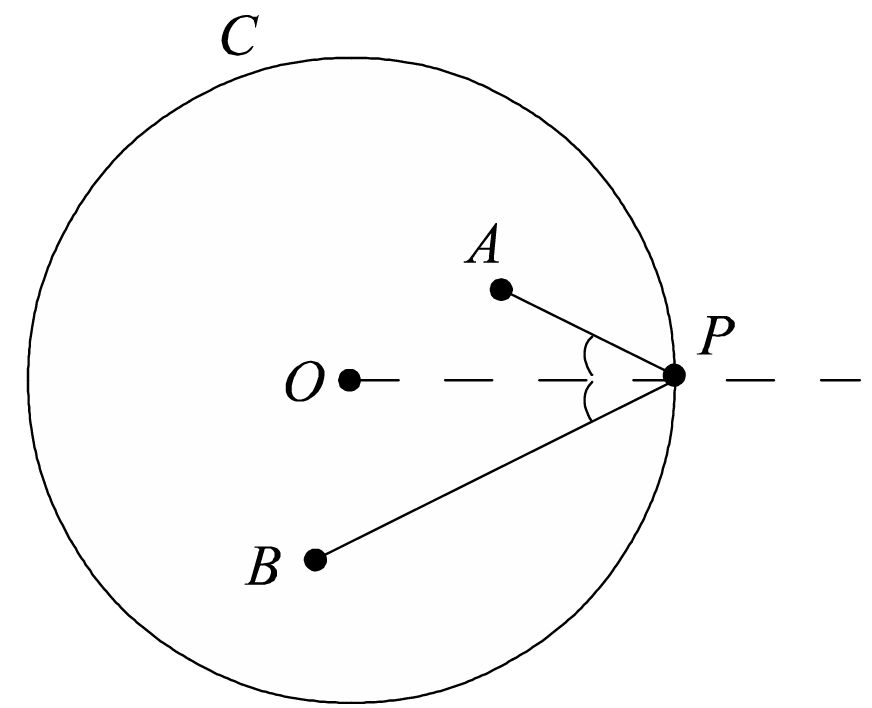
\includegraphics[width=0.4\textwidth]{images/alhazen/huygens1.png}
    \end{figure}
    Huygens in Nishimura: $A = a, B = b, P = z$. Potem velja
    $$ (ab) \overline{z}^2 - (\overline{ab}) z^2 = (a+b) \overline{z} - (\overline{a+b}) z. $$
\end{frame}

%------------------------------------------------

\begin{frame}{Reševanje}
    Naj bodo $q, p, r, s, x, y \in \mathbb{R}$ taka števila, da velja
    \begin{align*}
        ab &= q + i p, \\
        a + b &= r + i s, \\
        z &= x_0 + i y_0.
    \end{align*}
    Točka $P$ je presečišče krožnice $\mathcal{C}$ in hiperbole $\mathcal{Q}$ z enačbo $px_0^2 -2qx_0y_0 -py_0^2 - sx_0 + ry_0 = 0$.
    Če krožnico zavrtimo, da $x$-os razpolavlja kot $\angle AOB$, se nam enačba hiperbole poenostavi v $2qxy + sx - ry = 0$
    Iščemo skupne tangente njunih dualov
    $$ \mathcal{C^*}: x^2 + y^2 - 1 = 0 \; \text{ in } \; \mathcal{Q^*}: r^2x^2 + 2rsxy + s^2y^2 + 4qrx - 4qsy + 4q^2 = 0. $$
\end{frame}

%------------------------------------------------

\begin{frame}{Nishimurijev origami postopek}
    \begin{enumerate}
        \item Prepognemo premico $OA$ in z $E$ označimo njeno presečišče s krožnico~$\mathcal{C}$.
        \item Prepognemo premico $AB$ in središče njene simetrale označimo z $M$.
        \item Skozi točki $O$ in $M$ prepognemo premico $D$. Presečišče poltraka $OM$ s krožnico $\mathcal{C}$ označimo z $E'$.
        \item Prepognemo premico $EB$.
        \item Prepognemo pravokotnico $l_1$ na premico $EB$ skozi točko $B$.
        \item Prepognemo pravokotnico $l_2$ na premico $l_1$ skozi točko $A$.
        \item Prepognemo premico $OB$ in presečišče s premico $l_2$ označimo z $G$.
        \item Prepognemo premico $MG$.
        \item Prepognemo pravokotnico $l_3$ na premico $MG$ skozi točko $M$.
        \item Prepognemo pravokotnico na premico $l_3$ skozi točko $E'$ in njeno presečišče s premico $OB$ označimo s $H$.
        \item Prepognemo premico skozi središče $O$, ki točko $H$ preslika na premico $D$ v točko $K$.
        \item Prepognemo premico skozi središče $O$, ki točko $B$ preslika na premico $OA$. Sliko točke $K$ čeznjo označimo s $F$.        
        \item Prepognemo tangento $p$ na krožnico $\mathcal{C}$, ki točko $F$ položi na premico $D$. Točka $P$ je dotikališče tangente $p$ s krožnico $\mathcal{C}$.
    \end{enumerate}
\end{frame}

\end{document}